\documentclass[
 paper=A4,pagesize=automedia,fontsize=12pt,
 BCOR=15mm,DIV=22,
 twoside,headinclude,footinclude=false,
 english,fleqn,             % fleqn = linksbündige Ausrichtung von Formeln
 bibtotocnumbered,          % Literaturverz. im Inhaltsverz. eintragen
 liststotoc,                % Abbildungsverz. im Inhaltsverz. eintragen
 listsleft,                 % Abbildungsverz. an der längsten Nummer ausrichten
 pointlessnumbers,          % kein Punkt nach Überschriftsnummerierung
 cleardoublepage=empty      % Vakatseiten ohne Paginierung
]{scrbook}
\setlength\parindent{0em}

% Kodierung, Schrift und Sprache auswählen
\usepackage[utf8]{inputenc}
\usepackage[T1]{fontenc}
\usepackage[english]{babel}
% damit man Text aus dem PDF korrekt rauskopieren kann
\usepackage{cmap}
% Layout: Kopf-/Fußzeilen, anderthalbfacher Zeilenabstand
\usepackage{scrlayer-scrpage} \pagestyle{scrheadings}
                      \clearscrheadfoot
                      \ihead{\headmark}\ohead{\pagemark}
                      \automark[subsection]{section}
                      \setheadsepline{0.5pt}
\usepackage{setspace} \onehalfspacing
\usepackage{enumitem} \setlist{itemsep=0pt}
\deffootnote{1em}{1em}{\textsuperscript{\thefootnotemark }}
% clickable references
\usepackage{hyperref}
% Grafiken, Tabellen, Mathematikumgebungen
\usepackage[dvipsnames]{xcolor}
\usepackage{graphicx}
\usepackage{svg}
%\hypersetup{
%	colorlinks,
%	linkcolor={PineGreen},
%	citecolor={cyan!80!black},
%	urlcolor={blue!80!black}
%}
\usepackage{wrapfig}
\hypersetup{hidelinks}
\usepackage{tabularx, booktabs, makecell} \renewcommand{\arraystretch}{1.2}
\usepackage{amsmath,amsfonts,amssymb}
% Darstellung von Fließumgebungen
\usepackage{flafter,afterpage}
\usepackage[section]{placeins}
\usepackage[margin=8mm,font=small,labelfont=bf,format=plain]{caption}
\usepackage[margin=8mm,font=small,labelfont=bf,format=plain]{subcaption}
\usepackage{multicol}
\numberwithin{equation}{chapter}
\numberwithin{figure}{chapter}
\numberwithin{table}{chapter}

%%%%%%%%%%%%%%%%%%%%%%%%%%%%%%%%%%%%%%%%%%%%%%%%%%%%%%%%%%%%%%%%%%%%%%%%%%%%%%%%
% Ab hier ist Platz für eigene Ergänzungen (Pakete, Befehle, etc.)

% Dieses Paket liefert den Blindtext, der als Platzhalter in den Beispieldateien steht.
% Das kannst Du also entfernen, wenn Du den Blindtext nicht mehr brauchst.
\usepackage{lipsum}

\begin{document}
	
	
	% Titelpageseite
	\begin{titlepage}
		\begin{tabularx}{\linewidth}{X}
			
\includegraphics[width=6cm]{TU_Logo_SW} \\\hline\hline
			
			\vspace{4.5em}
			
			\begin{singlespace}\begin{center}\bfseries\Huge
					
					KZM on Si(1, 0, 0) Surface
					
			\end{center}\end{singlespace}
			
			\vspace{5.5em}
			
			\begin{singlespace}\begin{center}\large
					Master-Arbeit \\ zur Erlangung des Hochschulgrades \\
					Master of Science \\
					im Master-Studiengang Physik
			\end{center}\end{singlespace}\medskip
			
			\begin{center}vorgelegt von\end{center}
			\begin{center}
				{\large Andreas Weitzel} \\ geboren am 10.08.1999 in Fulda
			\end{center}\medskip
			
			\begin{singlespace}\begin{center}\large
					Institut für Theoretische Physik \\
					Fakultät Physik \\
					Bereich Mathematik und Naturwissenschaften \\
					Technische Universität Dresden \\ 2023
			\end{center}\end{singlespace}
		\end{tabularx}
	\end{titlepage}
	
	
	% Gutachterseite
	\thispagestyle{empty}\vspace*{48em}
	
	Eingereicht am xx.~Monat~20xx\vspace{1.5em}
	\par{\large\begin{tabular}{ll}
			1. Gutachter: & Prof.~Dr.~XX \\
			2. Gutachter: & Prof.~Dr.~YY \\
	\end{tabular}}
	
	
	% Abstractseite
	\newpage
	\begin{center}\large\bfseries Summary\end{center}
	
	
	Abstract \\
	English: \\
	
	\vspace{20em}
	Abstract \\
	Deutsch \\
	
	
	% Inhaltsverzeichnis
	
	%\cleardoublepage
	\tableofcontents
	
	
	
	% Hauptteil
	\mainmatter
	\renewcommand{\chapterautorefname}{Chapter}
	\renewcommand{\sectionautorefname}{Section}
	\chapter{Introduction}
	\section{Motivation}
	In the area of semiconductor technology, silicon has become the cornerstone material driving the innovations that power our modern world. Its versatility, reliability, and abundance have solidified its position as the basic building block of the semiconductor industry, making silicon responsible for large parts of the recent human revolution. Its semiconducting properties facilitate the creation of wafers and integrated circuits, which are the centerpieces of computers, smartphones, and virtually any recent electronic device. \\
	
	The most important part of integrated circuits are transistors. They function as switches which make up binary numbers and logic gates that every processor uses to do math. The speed at which processors perform calculations is majorly influenced by the number of transistors available. Therefore the pursuit of further miniaturization is crucial for performance enhancement. Up-to-date transistors approach wire diameters of about $5\text{ nm}$. (reference?) This is close to atomic scales as the diameter of a silicon atom and the lattice constant are around $0.2\text{ nm}$ or $0.55 \text{ nm}$ respectively. At these scales surface effects play an ever-increasing role in influencing the behavior and conductivity of the wires. Indeed manufacturers have difficulties controlling the current flow through the channels of the transistors. Hence a better understanding of the behavior of the surface is critical to ensure progress in classical computing. \\
	
	Specifialy the Si(001) surface of monocrystalline silicon is important because it forms an interface with the oxide layer in transistors, that isolates silicon wires from their environment. Also wafers are cut along the Si(001) surface. The orientation of the cut is important since many of a crystal's structural and electronic properties are highly anisotropic. \\
	
	The Si(001) surface undergoes an order-disorder phase transition between two surface reconstructions. While static properties like possible reconstructions, their energies and electronic structures are thoroughly investigated, the dynamic properties are not yet well understood. A rich dynamic phenomenon to consider is the Kibble-Zurek mechanism which describes the unavoidable non-adiabatic evolution of systems as they cross phase boundaries. The quench time is directly related to the number of domains of different order which in turn influence the electronic properties of the surface. \\
	
	\section{Thesis Structure}
	This thesis aims to contribute to the understanding of the dynamic behavior of Si(001) during a quench. The already existing discrete Ising-like description of the surface is extended to a continuous XY-like model and adapted to the silicon surface. Well established molecular dynamics methods are used in combination with state-of-the-art parallel programming and GPU acceleration techniques to overcome the numerous numerical obstacles that are inherent to the nature of phase transitions. The used Langevin-type stochastic differential equations are motivated from a quantum mechanics point of view. Renormalization group techniques are employed to set a theoretical baseline for the investigation of the phase transition. \\
	
	\autoref{Section::Silicon} firmly concludes the current viewpoint on and knowledge of the Si(001) surface and its order-disorder phase transition. \autoref{Chapter::Phase-Transitions} explores the renormalization group description of phase transitions to create a theoretical understanding for what follows. It introduces the concept of universality and the methods of finite size scaling which are used to investigate and interpret the simulation results.  \autoref{Chapter::Simulating-Dynamics} explains the used numerics and motivates our description from a quantum point of view. Moreover, the XY model used to describe the Si(001) surface is introduced and investigated. The results of various investigations like dynamic quenches, but also static measurements are written in \autoref{Chapter::Implementation-Results}. In \autoref{Chapter::Summary-Lookout} the main points of the thesis are summarized and an outlook for possible further research is given. The appendix contains calculations to various parts of the work as well as benchmarks for the simulation. \\
	
	The simulation is written in \texttt{C++} using \texttt{CUDA} \cite{cuda} and \texttt{Thrust} \cite{thrust}. The evaluation and plotting is done in \texttt{python}. The whole source code can be obtained at \texttt{github.com}.
	
	The surface is semiconducting \cite{himpsel1979photoemission, uhrberg1981experimental, handa1989plasma} \\
	
	
	\chapter{The Si(001) Surface} \label{Section::Silicon}
	\section{Surface Reconstruction}
	Below a temperature of $T =	1687~\text{K}$ silicon crystallizes in a diamond cubic crystal structure as shown in \autoref{Fig::SiliconDiamond} with a lattice constant of $a =	5.431~\text{\AA} $ \cite{tiesinga2021codata}. When cutting this crystal structure along the crystallographic (001) plane, the resulting system exhibits a surface reconstruction. Surface atoms are left in a high-energy state with two dangling bonds. One of those bonds can be invested into forming a dimer with the neighboring Si atom in (110) direction \cite{chadi1979atomic}, which, as shown by theoretical calculations \cite{ramstad1995theoretical, batra1990atomic, dabrowski1992self}, leads to a large reduction of surface energy of roughly $1.8~\text{eV}$ per dimer.
	\begin{figure}[htp]
		\centering
		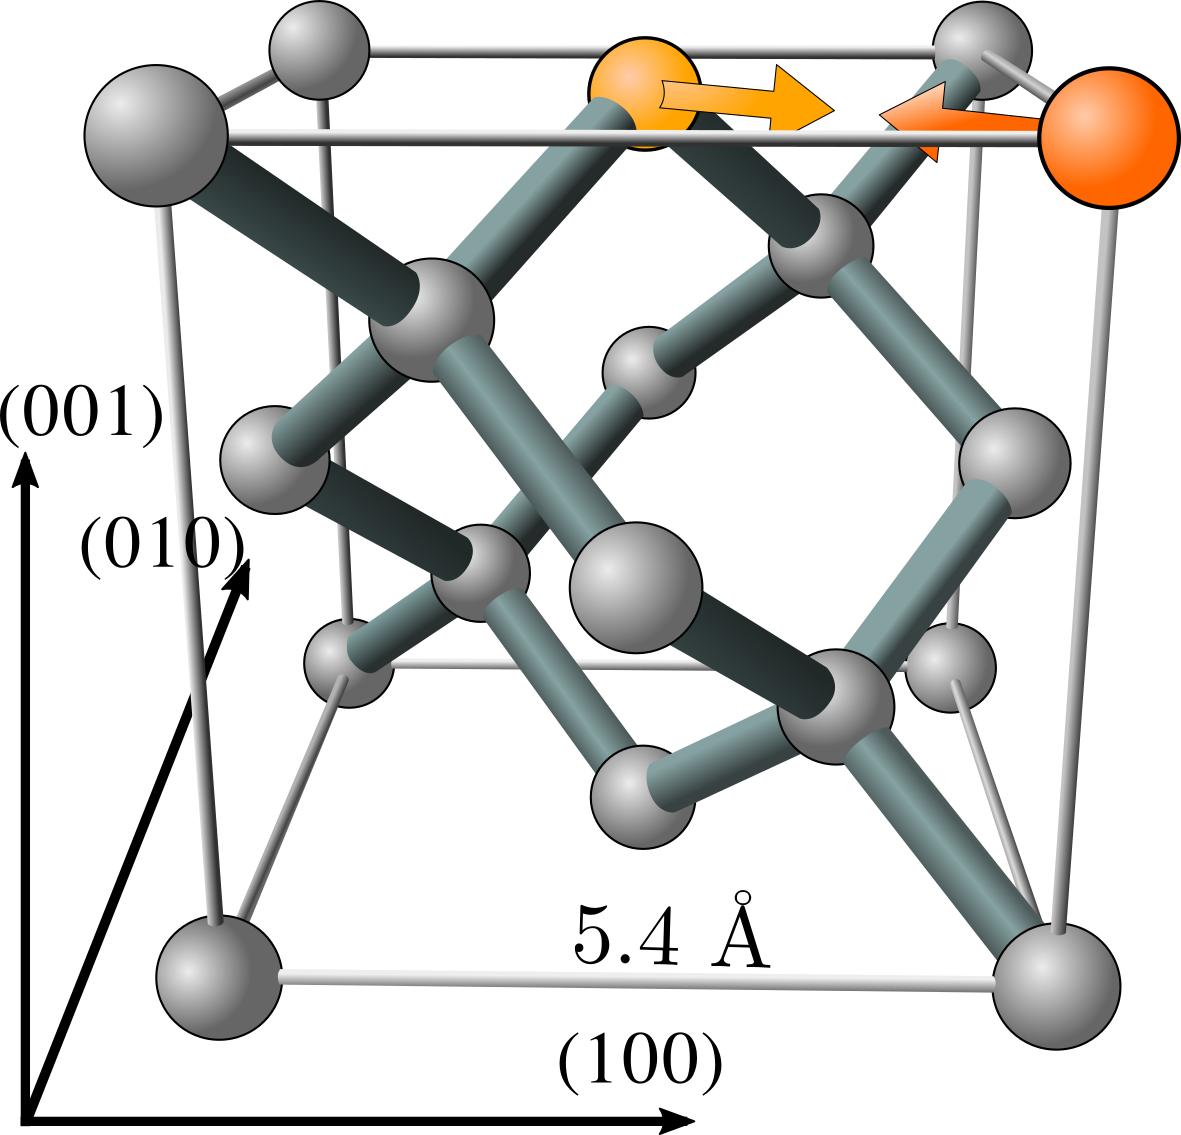
\includegraphics[width=0.5\linewidth]{graphics/Sili.png}
		\caption{The crystalline structure of Si in its solid state is shown \cite{sistrucure}. The orange colored atoms form a dimer when cutting the diamond structure along the (001) plane. The coordinate system axis are denoted by their Miller indices and normal to their corresponding crystallographic planes. The orange silicon atoms dimerize during reconstruction of the (001) surface.}
		\label{Fig::SiliconDiamond}
	\end{figure}
	
	The resulting dimers can further reduce their energy by vertical buckling. The dimers tilt to an angle of about $18^\circ$ \cite{ramstad1995theoretical, pillay2004revisit}, which lowers the surface energy by another $0.15~\text{eV}$ \cite{inoue1994order} per dimer. A charge transfer of approximately $0.1 e$  \cite{brand2023critical, landemark1992core} is induced by the buckling. The electrostatic interaction of the dimers is characterized by a coupling strength $J$. The surface reconstruction with the lowest energy was through theoretical \cite{ramstad1995theoretical, pillay2004revisit, inoue1994order, brand2023critical} and experimental (low energy electron diffraction \cite{matsumoto2003low, kubota1994streak, brand2023critical} and scanning tunnel microscope \cite{wolkow1992direct, tochihara1994low})  methods found to be the $c(4\times 2)$ reconstruction, shown in \autoref{Fig::dimer-configs} (b). It minimizes the interaction energy as well as the surface stress. The alternative buckling in both directions suggests an antiferromagnetic interaction along $(110)$, $J_\parallel$, and across $(1\overline{1}0)$, $J_\perp$, the dimer rows, but the interaction across the row is actually ferromagnetic. However, the dimer interactions are strongly anisotropic with $J_\parallel$ being much larger than $J_\perp$ which causes a guaranteed alternating buckling in $(110)$ direction. The ferromagnetic diagonal interactions $J_\times$ overpower $J_\perp$ so diagonal alignment is preferred, which in turn implies anti-alignment in $(1\overline{1}0)$ direction. It has been suggested that the interaction is of dipole kind \cite{pillay2004revisit}.
	\begin{figure}[htb]
		\begin{subfigure}{0.5\textwidth}
			\centering
			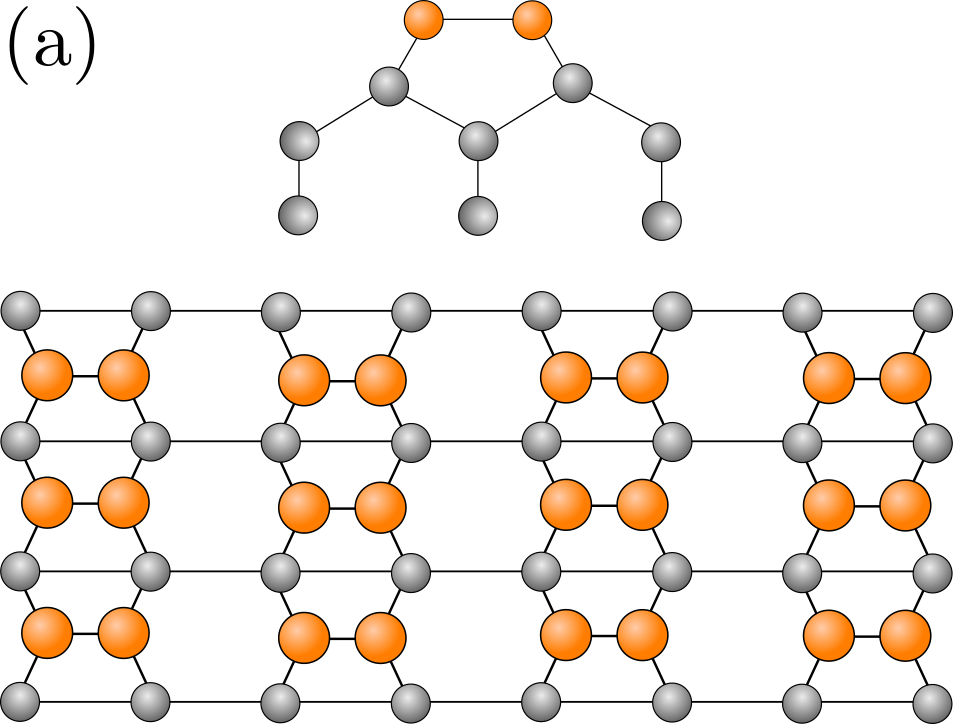
\includegraphics[width=0.8\textwidth]{graphics/p(2x1)-sym.png}
			\label{p(2x1)-symmetric}
		\end{subfigure}
		\begin{subfigure}{0.5\textwidth}
			\centering
			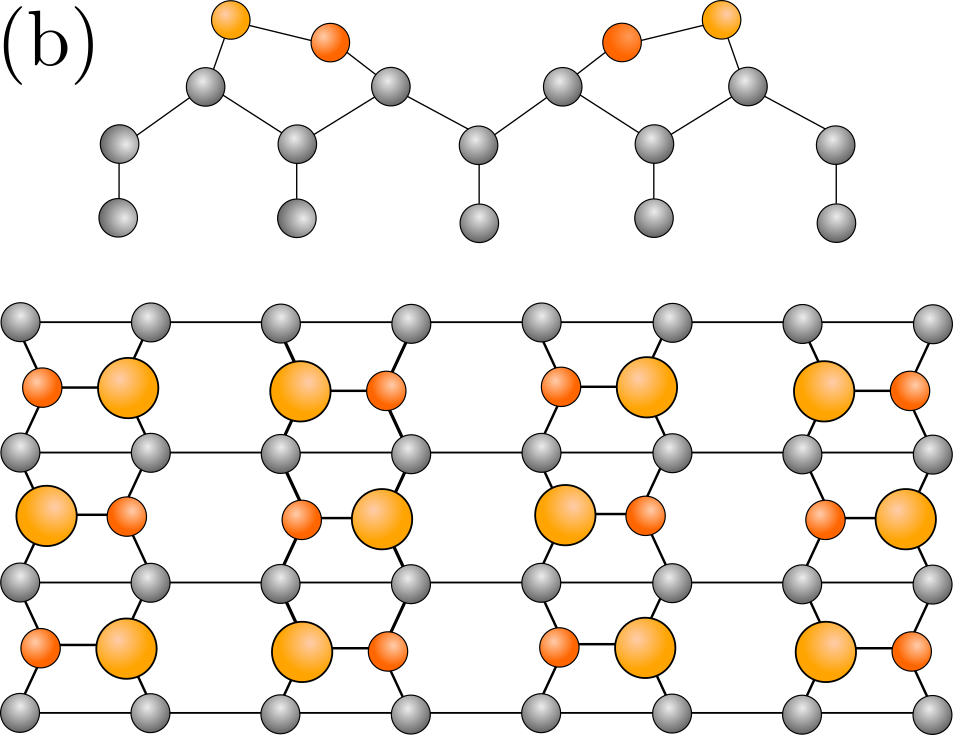
\includegraphics[width=0.8\textwidth]{graphics/c(4x2).png}
			\label{c(4x2)}
		\end{subfigure}
		\caption{ \textbf{(a)}The formation of dimers results in the symmetric $p(2\times1)$ reconstruction and saves a large amount of $1.8~\text{eV}$ per dimer compared to the ideal $p(1\times1)$ structure. \textbf{(b)} The dimers are unstable to vertical buckling. The buckling pattern that was found to have the lowest surface energy is the $c(4\times2)$ reconstruction.}
		\label{Fig::dimer-configs}
	\end{figure}
	\section{Phase Transition of the Si(0,0,1) Surface}
	The Si(001) surface exhibits an order-disorder phase transition from the disordered $p(2\times1)$ phase shown in \autoref{Fig::dimer-configs} (a) to the ordered $c(4\times2)$ reconstruction at a critical temperature of about $T_c \approx 200~\text{K}$ \cite{tabata1987order}. This continuous phase transition will be of central importance in the following discussion. The $p(2\times1)$ structure is short term for the disordered phase since fast flipping of the dimers at a frequency of about $ 10^{-11} \text{ Hz}$ let the system appear to be in the $p(2\times1)$ state at high-temperature measurements. \\
	
	The strong anisotropy leads to long streaks of order along the dimer rows ($\parallel$) and short domains of order across the dimer rows ($\perp$) . Brand et. al \cite{brand2023dimer} found that the ratio of correlation length amplitudes $\xi^+$ is ${\xi_{\parallel}^+}/{\xi_{\perp}^+} \approx 5.2$. The lattice spacing along the dimer rows is $a_\parallel =	3.84~\text{\AA}$, while it is $a_\perp =	2 a_\parallel =	7.68~\text{\AA}$ across. \\
	
	To understand the phase transition of the Si(001) surface we need to have a general knowledge of phase transitions.
	\chapter{Phase Transitions} \label{Chapter::Phase-Transitions}
	
	The term phase transition describes the process of transition between states of a system by changing an external parameter, like pressure $p$ or temperature $T$. Common types are transitions from an unordered to an ordered state after cooling a system below its critical temperature $T_c$ like the transition from paramagnets to ferromagnets. Intuitively the transitions happen as a result of free energy $F =	U - TS$ minimization. At high temperatures entropy $S$ dominates, leading to unordered states, but at low temperatures the impact of the internal energy $U$ takes over. The minimization of $U$ usually leads to a form of ordering dictated by the microscopic Hamiltonian. \\
	
	%A common type of phase transition is order-disorder transitions when the critical temperature $T_c$ of the system is exceeded, like the transition from ferromagnets to paramagnets. Phenomenologically one could say that the driving force behind the phase transition is the minimization of the free energy $F = U - TS $, with internal energy $U$ and entropy $S$. Below the critical temperature, the internal energy U is minimized leading to a form of ordering dictated by the microscopic Hamiltonian.
	\textbf{Mathematical definition:}
	
	Let $N$ denote the number of components, or equivalently the number of lattice sites, and $V$ the volume of the system in question. The \textbf{thermodynamic limit} $N \rightarrow \infty$ and $V \rightarrow \infty$ describes the limit to infinitely large systems while keeping the density $N/V$ constant. For a system dependent on a set of coupling constants $[K]$ the free energy per site $f$ is defined as
	%In the \textbf{thermodynamic limit} (system volume $V \rightarrow \infty$ or number of sites $N \rightarrow \infty$), we can give a mathematical definition of a phase transition. Consider our system to be dependent on a set of coupling constants $[K]$, which for example can be temperature $T$, pressure $p$ or interaction strength $J$. We define the free energy per site as
	\begin{equation}
		f[K] =	\lim\limits_{N \rightarrow \infty} \frac{F[K]}{N} ~.
	\end{equation}
	%If the thermodynamic limit exists,
	With $f$ a precise definition of the phase boundary is possible. The $d$ coupling constants $[K]$ span the so called phase space. In this $d$-dimensional phase space, the free energy density $f$ is analytic almost everywhere except from the possibility of non-analyticities at certain points, lines, planes, etc. up to dimensionality $d-1$. The connected areas of analyticity are called \textbf{phases} and non-analyticitys with dimension $d-1$ are called \textbf{phase boundaries} or \textbf{critical manifolds}. Since $f$ has to be continuous everywhere, the phase boundaries come in two classes:
	\begin{enumerate}
		\item at least one of the first derivatives $\frac{\partial f}{\partial K_i}$ is discontinuous across the phase transition. This case belongs to the \textbf{first-order phase transition}.
		\item all derivatives $\frac{\partial f}{\partial K_i}$ are continuous. This transition is called the \textbf{continuous phase transition}.
	\end{enumerate}
	The phase transition of the silicon surface belongs to the continuous phase transitions. As the thermodynamic limit is never obtained, descriptions using $f$ are not always reliable. Using the correlation length $\xi$, which simply put describes the spatial extent of fluctuations in the system, a criterion for accurate predictions can be given. If the system size $L$ is much greater than the correlation length $\xi \ll L$ the considered system can be expected to behave according to the ideal behavior described by $f$. \\
	%	The free energy density gives reasonable predictions, when the correlation length $\xi$, which is basically the spatial extent of fluctuations in the system, is much smaller than the system size L, so $\xi \ll L$.
	
	Phase transitions exhibit rich phenomena like the divergence of the correlation length $\xi$ at the critical point. The reason for the universality of this behavior across different systems will be outlined in the next section with the help of renormalization group theory.
	\section{Renormalization Group Considerations} \label{Section::RG}
	The renormalization group (RG) theory is a general framework to study phase transitions and particle physics. It employs scale invariance arguments, meaning the self-similarity characteristics of systems at different length scales, to investigate their properties. In the following basic considerations as well as important results shall be presented briefly. \\
	\begin{figure}[t]
		\centering
		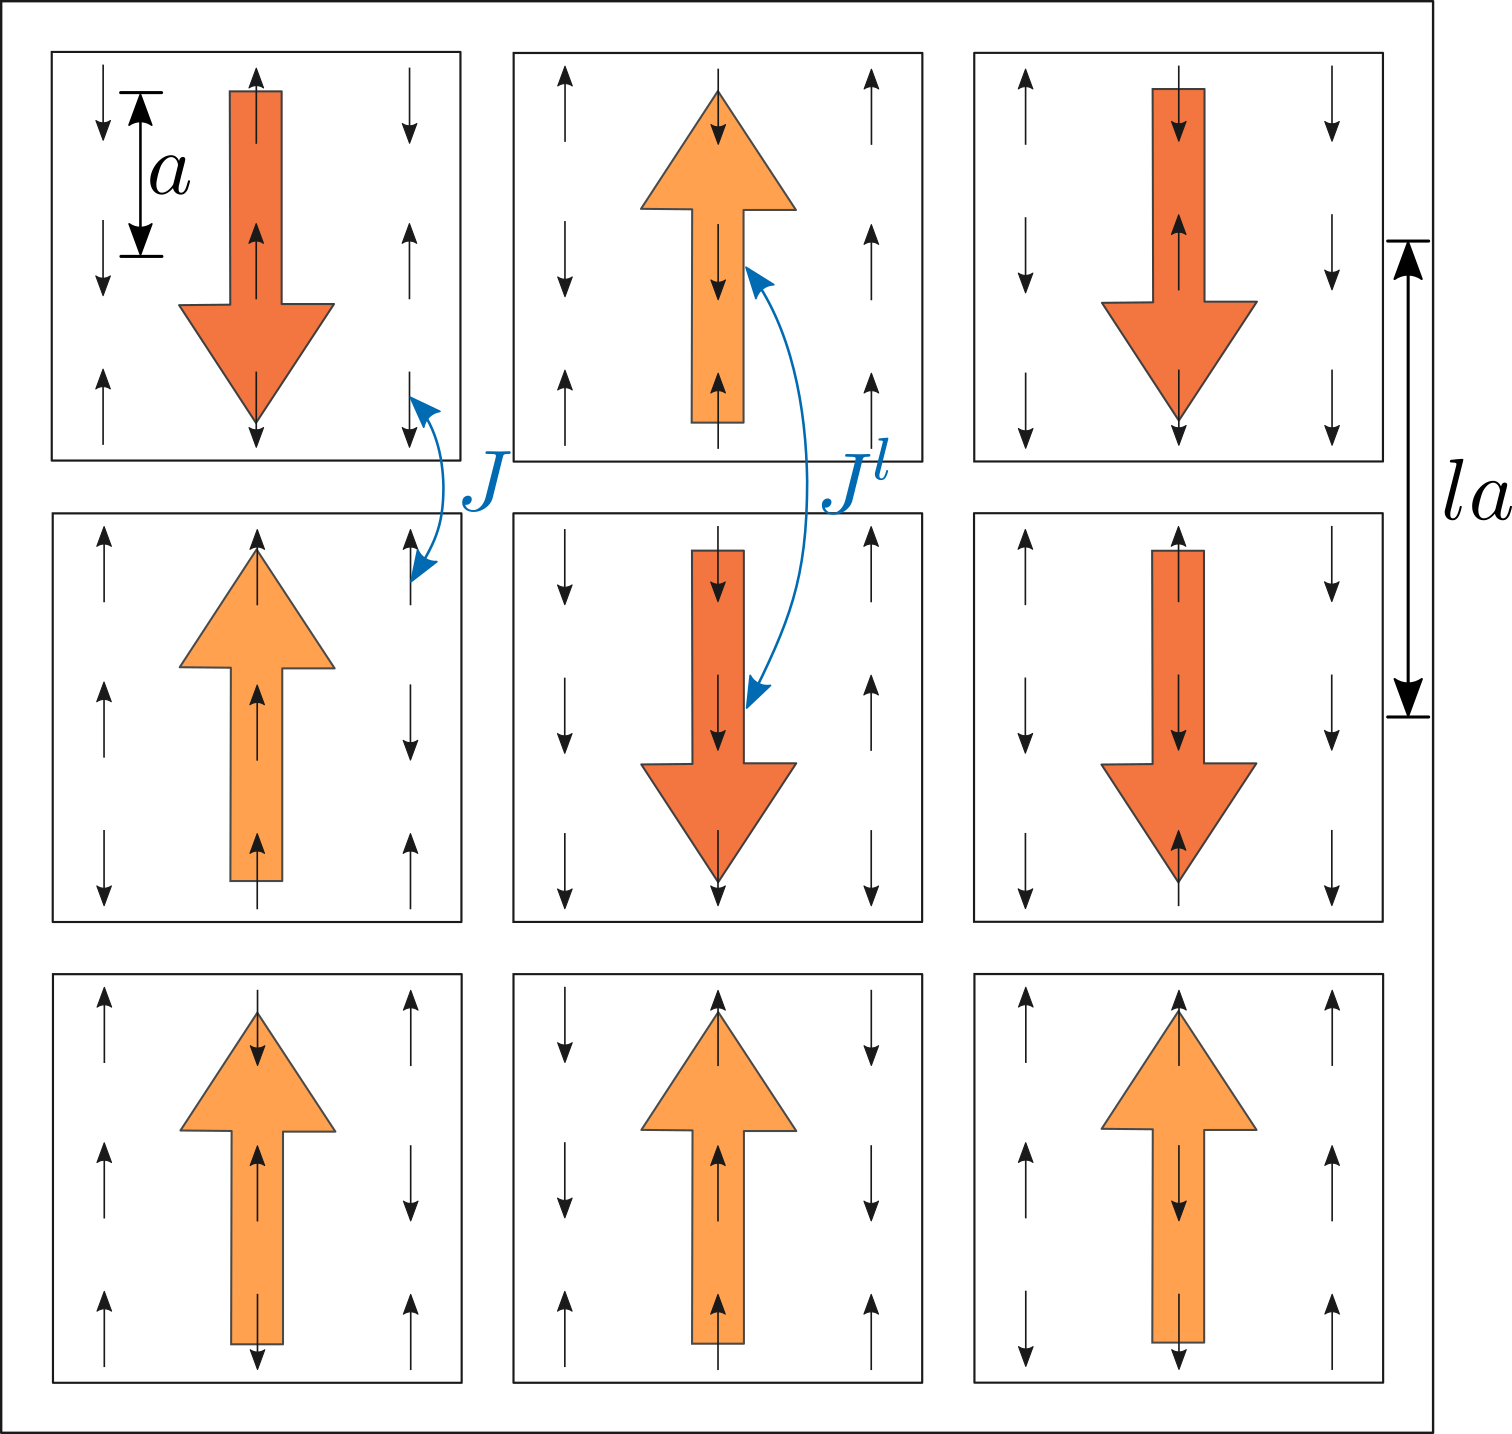
\includegraphics[width=0.7\linewidth]{graphics/RG-Iteration.png}
		\caption{In Kadanoffs block spin picture, $l^2$ Ising-spins are combined to a composite spin that takes on the value of the majority of spins. The block spin is the standard example for a renormalization group transformation. Under the RG transformation, the relevant length scales change from $a$ to $la$ and the coupling strengths from $J$ to $J^l =	R_l(J)$.}
		\label{Fig::RG-Iteration}
	\end{figure}
	
	Consider an infinite two-dimensional $d=2$ lattice with Ising-like spins $s_{mn}$ on each site. The site is denoted by a tuple of indices $(m,n)$. Following Kadanoff \cite{kadanoff1966scaling}, we examine a square of length $l$ in lattice spacing units $a$ and map  their combined $l^2$ spins to a single value $S^l$. This block spin is renormalized to $\pm 1$ by taking on the value of the majority of spins. The obtained $S_{ij}^l$ define a new Ising system, but on a different length scale with a new lattice spacing $la$ like shown in \autoref{Fig::RG-Iteration}. The proposal is that there exists a set of coupling parameters $[K^l]$ defining the interaction of the block spins so that the total free energy stays the same. In terms of the free energy density we can write
	\begin{equation} \label{free-energy-density}
		f[K] =	l^{-2} f[K^l]~,
	\end{equation}
	since the free energy density after the transformation has to increase by a factor $l^2$ as we measure in an $l$-times larger length scale. The same considerations are made for the correlation length, giving
	\begin{equation}
		\xi[K] = l \xi[K^l]~.
	\end{equation}
	Suppose we know how the coupling constants change under an RG transformation $R_l$
	\begin{equation}
		[K^l] =	R_l([K])~.
	\end{equation}
	This is the starting point to comprehend why phase transitions exhibit singular behavior. The idea is that even though the partition function
	\begin{equation}
		Z(\{K\})	= \sum_{\{s\}} e^{- \beta H(\{s\}, \{K\})}
	\end{equation}
	is a sum of exponentials which are analytic in $[K]$, the singularities can arise after an infinite number of RG iterations. Applying multiple RG transformations traces out a trajectory in coupling constant space $[K^{(l_1)}] \rightarrow [K^{(l_2)}]  \rightarrow ... \rightarrow [K^{(l_n)}]$ the \textbf{RG flow}. This trajectory is almost always attracted to fixed points. The behavior of a system near a fixed point is the origin of scaling and lets us extract important information, like the shape of the phase diagram.
	
	A fixed point of the RG	map satisfies
	\begin{equation}
		[K^{(*)}] =	R_l[K^{(*)}] ~.
	\end{equation}
	At this point the correlation length transforms according to
	\begin{equation}
		\xi[K^{(*)}] =	\xi[K^{(*)}] / l~,
	\end{equation}
	meaning that the correlation length either has to be $0$ or $\infty$. The same is true for the free energy density. In proximity of a fixed point we write the initial coupling constants as
	\begin{equation}
		K_i =	K_i^{(*)} + \delta K_i \qquad \text{and} \qquad K_i^l =	R_l(K_i^{(*)} + \delta K_i) =	K_i^{(*)} + \delta K_i^l~.
	\end{equation}
	The RG Transformation of $K_i$ is in general dependent on all $K$ so that
	\begin{equation}
		K^l_i =	K^l_i[K] =	K^l_i(K_1^{(*)} + \delta K_1, K_2^{(*)} + \delta K_2, ...).
	\end{equation}
	The Taylor expansion of $K_i^l$ around the fixed point $[K^{(*)}]$ yields the linearized RG Transformation
	\begin{equation} \label{linearized-RG}
		K_i^l =	K_i^{(*)} + \sum_j \frac{\partial K_i^l}{\partial K_j} \bigg |_{K_j = K_j^{(*)}} \delta K_j + O((\delta K_j)^2) = K_i^{(*)} + \delta K_i^l + O((\delta K_j)^2) ~.
	\end{equation}
	Omitting terms quadratic in $\delta K_j$ identifies
	\begin{equation}
		\delta K_i^l =	\sum_j \frac{\partial K_i^l}{\partial K_j} \bigg |_{K_j = K_j^{(*)}} \delta K_j~.
	\end{equation}
	We write down the partial derivatives as a matrix
	\begin{equation}
		M^l_{ij} =	\frac{\partial K_i^l}{\partial K_j} \bigg |_{K_j = K_j^{(*)}}~,
	\end{equation}
	and construct an eigenvalue problem
	\begin{equation} \label{ev-problem}
		M^l k^{(\sigma)} =	\lambda^{(\sigma)}_l k^{(\sigma)}~,
	\end{equation}
	where $\sigma$ labels the eigenvalues. Because two consecutive RG Transformations by $l_1$ and $l_2$ have to yield the same result as one  by $l_1l_2$, we know that
	\begin{equation}
		M^{l_1}M^{l_2} =	M^{l_1l_2}~,
	\end{equation}
	implying that
	\begin{equation}
		\lambda_{l_1}^{(\sigma)} \lambda_{l_2}^{(\sigma)} =	\lambda_{l_1l_2}^{(\sigma)} ~.
		\label{ev-equation}
	\end{equation}
	Setting $l_2 = 1$ gives $\lambda_{l_1}^{(\sigma)} \lambda_{1}^{(\sigma)} =	\lambda_{l_1}^{(\sigma)}$ which lets conclude that $\lambda_{1}^{(\sigma)} =	1$. Differentiating \autoref{ev-equation} with respect to $l_2$ yields
	%	\begin{equation}
		%		\begin{split}
			%			\frac{\text{d}}{\text{d}l_2} \left(\lambda_{l_1}^{(\sigma)} \lambda_{l_2}^{(\sigma)}\right) &= 	\frac{\text{d}}{\text{d}l_2} \lambda_{l_1l_2}^{(\sigma)} \\
			%			\lambda_{l_1}^{(\sigma)}  \left(\frac{\text{d}}{\text{d}l_2} \lambda_{l_2}^{(\sigma)}\right) +  			  \left( \frac{\text{d}}{\text{d}l_2} \lambda_{l_1}^{(\sigma)}\right) \lambda_{l_2}^{(\sigma)} &= l_1 \frac{\text{d}}{\text{d}(l_1l_2)} \lambda_{l_1l_2}^{(\sigma)} \\
			%			\left(\frac{\text{d}}{\text{d}l_2} \lambda_{l_2}^{(\sigma)}\right) \lambda_{l_1}^{(\sigma)}   &= l_1 \frac{\text{d}}{\text{d}(l_1l_2)} \lambda_{l_1l_2}^{(\sigma)}	~.
			%		\end{split}
		%	\end{equation}
	\begin{equation}
		\frac{\text{d}}{\text{d}l_2} \left(\lambda_{l_1}^{(\sigma)} \lambda_{l_2}^{(\sigma)}\right) = \lambda_{l_1}^{(\sigma)}  \left(\frac{\text{d}}{\text{d}l_2} \lambda_{l_2}^{(\sigma)}\right) +  			  \left( \frac{\text{d}}{\text{d}l_2} \lambda_{l_1}^{(\sigma)}\right) \lambda_{l_2}^{(\sigma)} 	= \left(\frac{\text{d}}{\text{d}l_2} \lambda_{l_2}^{(\sigma)}\right) \lambda_{l_1}^{(\sigma)}
	\end{equation}
	for the left hand side and
	\begin{equation}
		\frac{\text{d}}{\text{d}l_2} \lambda_{l_1l_2}^{(\sigma)} =	\frac{\text{d}}{\text{d}(l_2 l_1)} \lambda_{l_1l_2}^{(\sigma)} \frac{\partial}{\partial l_2} (l_1 l_2) =	l_1 \frac{\text{d}}{\text{d}(l_1l_2)} \lambda_{l_1l_2}^{(\sigma)}
	\end{equation}
	for the right hand side. By setting $l_2 =	1$ the differential equation
	\begin{equation}\label{RG-diff}
		\frac{\text{d}}{\text{d}l_2} \lambda_{l_2}^{(\sigma)} \bigg |_{l_2 =	1} \lambda_{l_1}^{(\sigma)}  = y_\sigma \lambda_{l_1}^{(\sigma)} = l_1 \frac{\text{d}}{\text{d}l_1} \lambda_{l_1}^{(\sigma)}
		%\quad \Rightarrow \quad \frac{\text{d}}{\text{d}l_1} \lambda_{l_1}^{(\sigma)} =	\frac{y_\sigma}{l_1} \lambda_{l_1}^{(\sigma)} ~.
	\end{equation}
	with
	\begin{equation}
		y_\sigma = \frac{\text{d}}{\text{d}l_2} \lambda_{l_2}^{(\sigma)} \bigg |_{l_2 =	1}
	\end{equation}
	is obtained.
	A solution to {\autoref{RG-diff}} is
	\begin{equation} \label{ev-form}
		\lambda_l^{(\sigma)} = l^{y_\sigma}~,
	\end{equation}
	with $y_\sigma$ being independent of $l$. This is an important result on the way to show the origin of scaling. The $k^{(\sigma)}$ are vectors in the coupling constant space, so \autoref{ev-problem} indicates that some $\delta K_i$ grow and some shrink when applying RG transformations, depending on the eigenvalue $\lambda_l^{(\sigma)}$. Three cases are distinguished:
	\begin{enumerate}
		\item \textbf{Relevant} directions and eigenvalues:	$|\lambda_l^{(\sigma)}| > 1$, meaning that $y_\sigma > 0$ and $\delta K$ in direction of $k^{(\sigma)}$ grow.
		\item \textbf{Irrelevant} directions and eigenvalues:	$|\lambda_l^{(\sigma)}| < 1$, meaning that $y_\sigma < 0$ and $\delta K$ in direction of $k^{(\sigma)}$ shrink.
		\item \textbf{Marginal} directions and eigenvalues:	$|\lambda_l^{(\sigma)}| = 1$, meaning that $y_\sigma = 0$ and $\delta K$ in direction of $k^{(\sigma)}$ do not change.
	\end{enumerate}
	After many iterations, only the relevant eigenvalues will be important, as shrinking $\delta K_i$ won't impact the RG flow significantly. If we differ from the fixed point in a relevant direction, the differences to the fixed point will become larger and the RG transformation flow will move away from the fixed point. Deviations in irrelevant direction will flow into the fixed point. \\
	
	A simplified understanding can be achieved for a system satisfying
	\begin{equation}
		\frac{\partial K_i^l}{\partial K_j} \bigg |_{K_j = K_j^{(*)}} = \delta_{ij} \frac{\partial K_j^l}{\partial K_j} \bigg |_{K_j = K_j^{(*)}}~,
	\end{equation}
	so that $M^l_{ij}$ becomes diagonal and the eigendirections $k^{(\sigma)}$ point directly along the axes $e^{K_i}$ of the phase space defined by $K$. If the eigenvalue $\lambda_l^{(\sigma)}$ to $k^{(\sigma)}$, parallel to $e^{K_i}$, is larger than one, the coupling $K_i$ will grow. In this case $K_i$ would be a relevant coupling constant. \\
	
	Consider a system with only one coupling constant, in this case the temperature, and choose $T$ in the vicinity of a fixed point $T^{(*)}$. Apply a RG transformation to $T$ and consider the difference
	\begin{equation} \label{temp-difference}
		T^l - T^{(*)} =	R_l(T) - T^{(*)}~.
	\end{equation}
	Using \autoref{linearized-RG} we can rewrite
	\begin{equation}
		R_l(T) =	T^{(*)} + \delta T^l =	T^{(*)} + \frac{\partial T^l}{\partial T} \bigg |_{T =	T^{(*)}} \delta T =	T^{(*)} + \lambda_l \delta T~,
	\end{equation}
	since $M^l$ has only one component and $\delta T$ is therefore automatically in eigenvector direction. \autoref{temp-difference} then becomes
	\def\equationautorefname{Eq.}
	\begin{equation} \label{coupling-constant-ev-scaling}
		\varepsilon^{(l)} =	\lambda_l \varepsilon \overset{\text{\autoref{ev-form}}}{=} \varepsilon l^{y_\varepsilon}~,
	\end{equation}\def\equationautorefname{Equation}
	in terms of the \textbf{reduced temperature} $ \varepsilon =	\frac{T - T^{(*)}}{T^{(*)}}$. After $n$ RG iterations this gives
	\begin{equation}
		\varepsilon^{(nl)} = \left( l^{y_\varepsilon}	\right)^n \varepsilon~.
	\end{equation}
	Now consider again how the correlation length transforms after $n$ RG transformations
	\begin{equation} \label{xi-behavior}
		\xi(\varepsilon) =	l^n \xi(\varepsilon^{nl}) =	l^n \xi( l^{ny_\varepsilon} \varepsilon)~.
	\end{equation}
	Substituting $\tau =	l^{ny_\varepsilon} \varepsilon$ into \autoref{xi-behavior} yields
	\begin{equation} \label{Eq::RG-xi-scaling}
		\xi(\varepsilon) =	\tau^{1 / y_\varepsilon} \varepsilon^{-1/ y_\varepsilon} \xi(\tau)~,
	\end{equation}
	showing that the correlation length diverges as $\varepsilon \rightarrow 0$. This is the origin of scaling and universality! Note that knowledge of a valid RG transformation $R_l$ directly provides knowledge of $y_\varepsilon$ via
	\begin{equation}
		y_\varepsilon =	\frac{1}{l} \ln \left(\frac{\partial R_l (T)}{\partial T} \bigg|_{T^{(*)}}\right)~.
	\end{equation}
	\section{Universality and Static Scaling} \label{Section::Universality}
	The last section traced the origin of universality and scaling in phase transitions. This section will deal with the term universality and its implications in more detail. \\
	
	Scaling laws like \autoref{Eq::RG-xi-scaling} can be derived for different system quantities. In the context of phase transitions, \textbf{static scaling} means the power law dependence of a system quantity \textbf{in equilibrium}, like the correlation length $\xi$, on a coupling parameter, like the temperature $T$. The exponent of this power law is called the \textbf{critical exponent}. Some important scaling relations are shown in \autoref{Table::Scaling-Laws}. Comparing the scaling law of $\xi$ with \autoref{Eq::RG-xi-scaling} identifies
	\begin{equation}
		\frac{1}{y_\varepsilon} = \nu ~.
	\end{equation}
	%	\begin{itemize}
		%		\item the specific heat $\boldsymbol{C_H}$: $T_c C_H \approx A^{\pm} |\varepsilon|^{-\alpha}$,
		%		\item the order parameter $\boldsymbol{\Psi}$ or $\boldsymbol{M}$: $|M| \approx B |\varepsilon|^{-\beta}$,
		%		\item the susceptibility $\boldsymbol{\chi}$: $\chi \approx C^{\pm} |\varepsilon|^{-\gamma}$,
		%		\item and the correlation length $\boldsymbol{\xi}$ : $\xi \approx f^{\pm} |\varepsilon|^{-\nu}$.
		%	\end{itemize}
	\begin{table}[h]
		\centering
		\caption{Some important scaling laws are summarized in the notation of \cite{pelissetto2002critical}. The universal critical exponents $\alpha, \beta,$ etc. are the same above and below the phase transition. In contrary, the nonuniversal critical amplitudes may differ at different sides of the critical point. Hence, they are labeled with a superscript $\pm$. The dimensionality is denoted by $d$.}
		\begin{tabular}{l c l}
			\toprule
			Name  & $\quad$ Symbol $\quad$ & Scaling \\
			\midrule
			specific heat & $C_H$ & $T_c C_H \approx A^{\pm} |\varepsilon|^{-\alpha}$ \\
			order parameter & $\Psi, M$ & $|M| \approx B |\varepsilon|^{-\beta}$ \\
			susceptibility & $\chi$ & $\chi \approx C^{\pm} |\varepsilon|^{-\gamma}$ \\
			correlation length & $\xi$ & $\xi \approx f^{\pm} |\varepsilon|^{-\nu}$ \\
			two-point correlation function & $C(\vec{r})$& $C(\vec{r}) \propto |\vec{r}|^{- d + 2 - \eta}$ \\
			\bottomrule
		\end{tabular}
		\label{Table::Scaling-Laws}
	\end{table}
	The prefactors of the power laws are called the \textbf{critical amplitudes} and $\nu, \alpha, $ etc. are the mentioned critical exponents. The superscript $\pm$ denotes whether the phase transition is approached from below $(-)$ or above $(+)$ the critical temperature $T_c$. The critical exponents are the same on both sides of the transition, but the amplitudes vary. \\
	
	These scaling laws are only valid in the thermodynamic limit for $\varepsilon \rightarrow 0$ as the derivation in \autoref{Section::RG} assumed that the system is in the vicinity of a critical point. Otherwise they exhibit \textbf{corrections to scaling} that result out of irrelevant and marginal eigenvalues of the RG transformations as well as \textbf{finite-size} corrections. \\
	
	Systems that share the same set of critical exponents belong to the same \textbf{universality class}. \autoref{Section::RG} showed that the exponents can be calculated solely from the RG transformation which suggests that systems with similar transformations exhibit similar critical behavior. Indeed it is found that the universality class of a system only depends on
	\begin{itemize}
		\item the \textbf{symmetry group} of the system Hamiltonian,
		\item the \textbf{dimensionality} of the problem,
		\item and whether the \textbf{interaction} between the components is \textbf{short-ranged}.
	\end{itemize}
	In contrast to the critical exponents, the critical amplitudes are not universal, but their ratios, for example $f^+/f^-$, are.\\
	
	The concept of universality is very useful to investigate real systems at the critical point. As a result of scale invariance and self similarity, the microscopic dynamics of a system become irrelevant at $\varepsilon =	0$. Its behavior can then be approximated by a simplified, in the best case exactly solvable, model. \\
	
	The extraction of critical exponents is notoriously difficult for various reasons, one being the inaccessibility of the thermodynamic limit, another \textbf{critical slowing down} (see \autoref{Section::Dynamic-Scaling}). The following section will explain the mentioned finite size corrections to static scaling and illustrate how they can be used to analyze critical exponents.
	\section{Finite-size Scaling and Critical Exponent Extraction} \label{Section::FSS}
	The system size $L$ transforms after RG transformation according to
	\begin{equation}
		R_l(L) =	L^{(l)} =	L /	l ~,
	\end{equation}
	analogous to the correlation length. Extending the transformation of the free energy density of \autoref{free-energy-density} by a dependence of the system size yields
	%	Recall how the free energy density \autoref{free-energy-density} transforms and that it depends on the system size $L = l L^{(l)}$:
	\begin{equation}\label{FSS-free-energy-scaling}
		f\left([K], L^{-1}\right) =	l^{-2} f\left([K^{(l)}], {L^{(l)}}^{-1}\right) = l^{-2} f\left([K^{(l)}], l{L}^{-1}\right)	 ~,
	\end{equation}
	the \textbf{finite-size scaling} (FSS) of $f$.
	Let $K_1 =	\varepsilon$ be the reduced temperature. Close to the critical point \autoref{coupling-constant-ev-scaling} can be used to write \autoref{FSS-free-energy-scaling} in terms of eigenvalues
	\begin{equation}
		f\left(\varepsilon, K_2, ..., L^{-1}\right) = l^{-2} f\left(\varepsilon l^{y_\varepsilon}, K_2 l^{y_2}, ..., l{L}^{-1}\right)	 ~.
	\end{equation}
	The system size behaves like a relevant coupling constant with an eigenvalue of
	\begin{equation}
		\lambda_L =	1~, \qquad \text{implying that} \qquad y_L =	1 ~.
	\end{equation}
	This means that the system size has to be tuned to criticality for the phase transition to occur. Like $\varepsilon$, the inverse system size has to be set zero $L^{-1} =	0$ which is equivalent to taking the thermodynamic limit. As a result, real, finite systems deviate from the behavior that scaling laws dictate. The actual correlation length cannot outgrow the system size $\xi_L \leq L$ and so the divergence of $\xi$ is rounded at the phase transition. Additionally,  the peak of $\xi_L(T)$ is shifted \cite{guton1983phase} (to a lower critical temperature?). The ideal behavior of $\xi$ is compared to the behavior of a finite system in  \autoref{xi-divergence-FS}. \\
	
	\begin{figure}[htp]
		\centering
		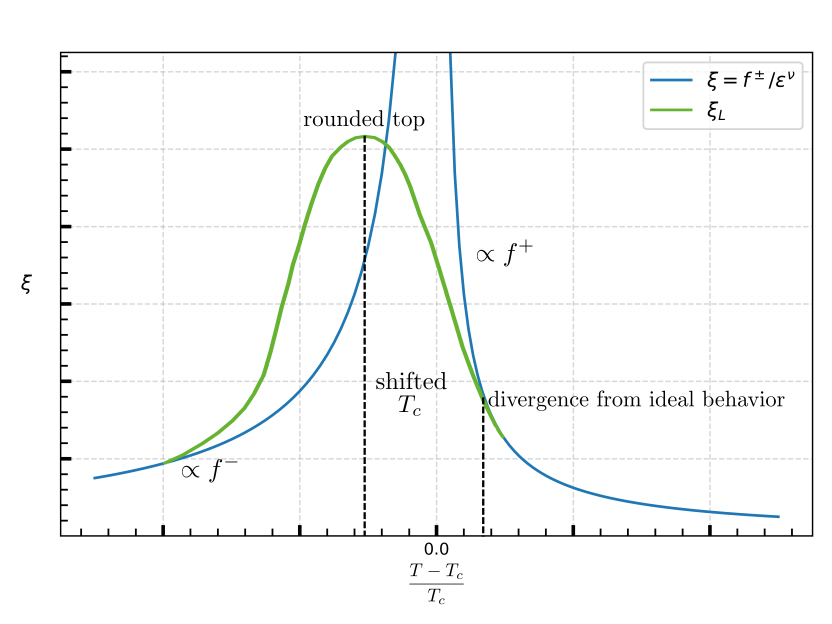
\includegraphics[width=0.7\linewidth]{graphics/xi-divergence4.png}
		\caption{The equilibrium correlation length $\xi$ is shown versus the reduced critical temperature. In the thermodynamic limit, $\xi$ diverges at the critical point according to a power law, as depicted by the blue line. For finite systems, the singularity of $\xi$ appears rounded as shown by the green curve. The peak position is shifted to an effective critical temperature.}
		\label{xi-divergence-FS}
	\end{figure}
	Now consider \autoref{xi-behavior} extended by $L$-dependence reading
	\begin{equation}
		\xi(\varepsilon, L^{-1}) =	l \xi (\varepsilon l^{y_\varepsilon}, l L^{-1}) = \varepsilon^{-\nu} F_\xi (L^{-1} \varepsilon^{-\nu})~,
	\end{equation}
	with $F_\xi$ as in \autoref{Eq::RG-xi-scaling}. Introducing a new scaling function $F' =	(L \varepsilon^\nu)^{-1} F_\xi$ yields
	\begin{equation}
		\xi(\varepsilon, L^{-1}) = \varepsilon^{-\nu} (L\varepsilon^\nu) F' (L \varepsilon^{\nu}) =	L	F'(L \varepsilon^\nu)~.
	\end{equation}
	In the limit $L \rightarrow \infty$ and close to $\varepsilon =	0$, $\xi$ has to scale like $\xi(\varepsilon, 0) \propto \varepsilon^{-\nu}$ implying that
	\begin{equation}
		\lim_{L \rightarrow \infty} \lim_{\varepsilon \rightarrow 0} F'(L \varepsilon^\nu) \propto (L \varepsilon^\nu)^{-1}~.
	\end{equation}
	The correlation length is capped for finite $L$ so that at the critical point $\xi(0, L^{-1}) \propto L$. For $F'$ this means
	\begin{equation}
		\lim_{\varepsilon \rightarrow 0} F'(L\varepsilon^\nu) \propto \text{const.}~,
	\end{equation}
	showing that the scaling function does not diverge. Therefore a Taylor expansion around $\varepsilon =	0$ is reasonable and gives
	\begin{equation} \label{Equation::FSS-Scaling-L/xi}
		\frac{L}{\xi(\varepsilon, L^{-1})} =	A + B \varepsilon L^{1/\nu} + O(\varepsilon^2)~. 
	\end{equation}
	This equation is an important result since it can be used to calculate two central quantities. Firstly, curves of $L/\xi(\varepsilon, L^{-1})$ for different $L$ intersect at the critical point $\varepsilon = 0$. Hence, by determining this intersection one can extract the critical temperature $T_c$, which is usually not known a priori. Secondly by computing the gradient
	\begin{equation}
		\frac{\partial}{\partial \varepsilon} \left(\frac{L}{\xi(\varepsilon, L^{-1})}\right) =	B L^{1/\nu}
	\end{equation}
	for various $L$, one can determine the critical exponent $\nu$. This method is easier than, for example, trying to fit to the original scaling law \autoref{Eq::RG-xi-scaling} because of the reasons mentioned at the end of \autoref{Section::Universality}.
	\subsection{Binder Cumulant} \label{Sec::Binder-Cumulant}
	FFS scaling laws like \autoref{Equation::FSS-Scaling-L/xi} can be derived for any thermodynamic quantity \cite{pelissetto2002critical, blote1995ising}. The Binder cumulant $U_L$, introduced by K. Binder in \cite{binder1981finite}, is frequently used to investigate simulations. It is defined as
	\begin{equation} \label{Eq::Def-Binder-Cum}
		U_L =	\frac{\langle M_L^4 \rangle}{\langle M_L^2 \rangle^2}~,
	\end{equation}
	with $M_L$ being the order parameter of a system of size $L$. The ensemble average $\left\langle~\cdot~\right \rangle$ denotes the mean of infinitely many system realizations. Its finite size scaling is analogous to \autoref{Equation::FSS-Scaling-L/xi} given by
	\begin{equation}
		U_L =	U^* + U \varepsilon L^{1/\nu} \left(1 + W L^{-\omega} + ...\right)~,
	\end{equation}
	including corrections resulting out of the largest irrelevant eigenvalue $1/|y_1| =	\omega $.
	To extract the critical exponent $\nu$ a linear fit to
	\begin{equation} \label{Eq::FSS-dU_dT}
		\ln \left(\frac{\partial U_L}{\partial \varepsilon}\right) \approx	\ln \left(U L^{1/\nu} \right) =	\ln (U) + \frac{1}{\nu} \ln (L) ~.
	\end{equation}
	is performed.
	The Binder cumulant has a value of $U_L=1$ far below the phase transition, approaches $U_L =	3$ above the phase transition and exhibits the intersection in between at $U_L =	U^*$. It is generally easy to compute and extract.
	\section{Dynamic Scaling and the Kibble-Zurek Mechanism} \label{Section::Dynamic-Scaling}
	\subsection{The Relaxation Time $\tau$ and the Critical Exponent $z$}
	With the Binder cumulant we acquired a way to extract the static scaling exponent $\nu$. Aside static scaling, \textbf{dynamic critical phenomena} are of central importance to describe phase transitions. Dynamic scaling describes how much time fluctuations in systems take to equilibrate. This time is called the  \textbf{relaxation time} $\tau_k$ and it is usually specified for different lengthscales with the wavenumber $k$. The zero wavenumber relaxation time $\tau_0 =	\tau$ quantifies relaxation on the largest lengthscales. Its scaling \cite{hohenberg1977theory}
	\begin{equation}
		\tau =	\tau_\xi \xi(\varepsilon)^z
	\end{equation}
	defines a new \textbf{dynamic critical exponent} z. (TODO RG explanation for this scaling?). \\
	
	Plugging in the known scaling of $\xi(\varepsilon)$ from \autoref{Section::Universality} yields
	\begin{equation}
		\tau = \tau_\xi \xi(\varepsilon)^z =\tau_\xi	\left(f^{\pm} |\varepsilon|^{-\nu}\right)^z :=	\tau_\varepsilon |\varepsilon|^{-\nu z} ~.
	\end{equation}
	As the correlation length diverges, so does the relaxation time. Interpreting $\xi$ as a characteristic length at which system components are still influenced by each other gives an intuitive explanation for this divergence. The maximum speed for the propagation of interactions in the system is the respective speed of sound. Even the speed of sound would need an infinite amount of time to cover an infinite distance. In practice the propagation will take much more time. This is the in \autoref{Section::Universality} mentioned phenomenon of critical slowing down. As a system approaches $\varepsilon \rightarrow 0$, it takes longer and longer to equilibrate. It then becomes a computational challenge to let large systems equilibrate. But since static scaling laws describe quantities in equilibrium and are only valid in the thermodynamic limit for $\varepsilon \rightarrow 0$, large, critical systems have to be considered.  This dilemma was partially solved by the finite size techniques of \autoref{Section::FSS}. \\
	
	As well as its complementary static phenomenon does the dynamic scaling exhibit universality. The static and dynamic universality classes are not independent, but the dynamic ones form subgroups of the static universality classes. Besides the usual indicators described in \autoref{Section::Universality}, the conservation laws that are fulfilled by the system, as well as Poisson-bracket relations between the order parameter and the conserved densities are decisive for the respective universality class. The important anisotropic Ising model is part of Model A as specified by Hohenberg and Halperin \cite{hohenberg1977theory}. Its dynamic critical exponent can be expressed in terms of
	\begin{equation} \label{Eq::Model-A-z}
		z =	2 + c \eta ~,
	\end{equation}
	with $\eta$ as in \autoref{Table::Scaling-Laws} and $c$ a constant to be determined.
	\subsection{Quenches and the Freezeout of Domains}
	Systems like the Si(001) surface that exhibit order-disorder phase transitions usually have multiple possible orderings in the low temperature state. Boundaries between domains of different order, also called domain walls, are stable topological defects. The \textbf{Kibble-Zurek mechanism} (KZM) \cite{kibble1976topology, zurek1985cosmological, zurek1996cosmological} describes the final density of topological defects after driving a system through its phase transition. It directly relates the correlation length to the static and dynamic critical exponents $\nu$ and $z$ through a scaling law that has been verified in numerous experiments \cite{ruutu1996vortex, ulm2013observation, pyka2013topological}. The KZM shall be a central point of the upcoming investigations and will be explained in the following. \\
	
	We will solely consider linear quenches, concretely the cooldown of a system linear in time $t$. The speed of cooling is characterized by the \textbf{quench timescale} $\tau_Q$ defined by
	\begin{equation} \label{Eq::Linear-Quench}
		\varepsilon(t) =	\frac{t}{\tau_Q}~.
	\end{equation}
	For slow quenches sufficiently far away from the critical point, the system will evolve adiabatically, meaning that thermodynamic quantities like $\xi$ assume their equilibrium values. As the system approaches the phase transition at $t=0$, the derivative
	\begin{equation}
		\frac{\partial}{\partial t} \xi(\varepsilon(t)) =	- \nu f^{\pm} \frac{(\tau_Q)^\nu}{t^{-(\nu + 1)}}
	\end{equation}
	diverges and at some point will eventually outgrow the reaction capability of the system. The actual correlation length will diverge from its equilibrium behavior like shown in \autoref{Fig::Freezeout}. The timepoint $\hat{t}$ of divergence from the equilibrium behavior is called the \textbf{freezeout} since the current state of the system effectively becomes frozen in comparison with the equilibrium values. The KZM states that the freezeout roughly happens at
	% when the current relaxation time $\tau$ equals the time until the crossing of the critical point $\hat{t}$, defining
	\begin{equation}
		\tau(\hat{t}) = \hat{t}~,
	\end{equation}
	so as soon as $\tau$ exceeds the time that is left until the critical point is crossed.
	\begin{figure}[t!]
		\centering
		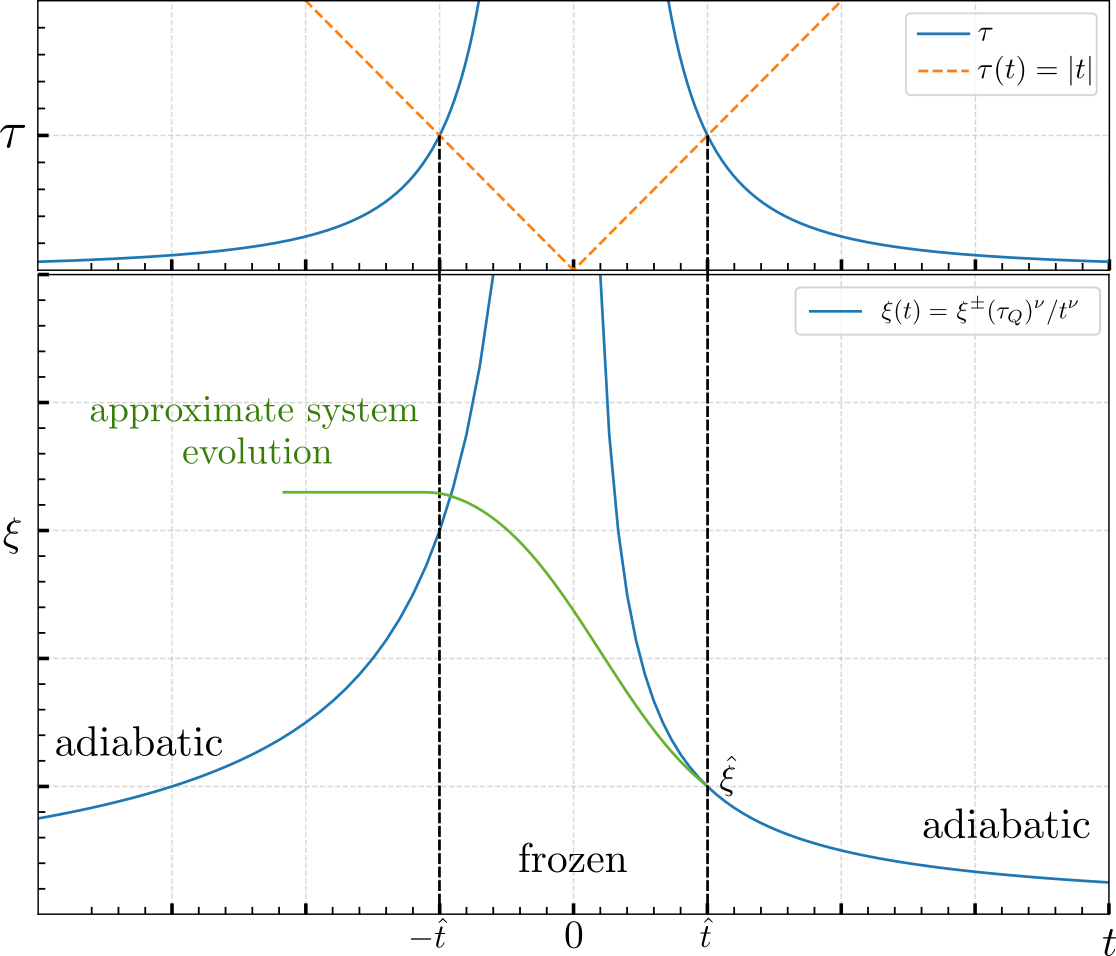
\includegraphics[width=0.7\linewidth]{graphics/KZM-divergences.png}
		\caption{In the top plot the divergence of the relaxation time $\tau$, i.e. the critical slowing down, is shown in blue versus the time $t$ during a linear quench. The freezeout of the current state happens roughly at $\tau(\hat{t}) =	\hat{t}$, visualized by the intersection with the dotted orange line. In the bottom plot the divergence of the equilibrium $\xi$ on the quench time is shown. Before $\hat{t}$ a quenched system evolves approximately adiabatic, following the blue line. After the freezeout, the actual correlation diverges from the equilibrium behavior, shown by the green line. Note that in this parameterization, a cooling quench runs from $t > 0$ to $t < 0$. The frozen domain walls are topologically stable in time.}
		\label{Fig::Freezeout}
	\end{figure}
	The system quantities after the quench will be directly related to their equilibrium values at $\hat{t}$. Combining
	\begin{equation}
		\hat{t} =	\varepsilon(\hat{t}) \tau_Q \qquad \text{and} \qquad  \hat{t} =	\tau(\hat{t}) = \tau(\varepsilon(\hat{t})) =	\tau_\varepsilon \big | \varepsilon(\hat{t}) \big |^{-\nu z}
	\end{equation}
	yields the reduced temperature at $\hat{t}$
	\begin{equation}
		\big|\varepsilon (\hat{t}) \big| =	\left(\frac{\tau_\varepsilon}{\tau_Q} \right)^{\frac{1}{1 + \nu z}} ~.
	\end{equation}
	For the scaling of $\xi$ this means
	\begin{equation} \label{Eq::KZM-scaling}
		\xi \propto \hat{\xi} := \xi(\varepsilon(\hat{t})) =	\xi_0 / |\varepsilon(\hat{t})|^{\nu} =	\xi_0 \bigg| \frac{\tau_Q}{\tau_\varepsilon} \bigg |^{\frac{\nu}{1 + \nu z}} ~,
	\end{equation}
	so the frozen value of the correlation length scales with the quench timescale like $\hat{\xi} \propto \tau_Q^{\frac{\nu}{1 + \nu z}}$~.
	The freezeout of the correlation length implies domains of order with an extent proportional $\hat{\xi}^2$. The domain walls separating ordered areas may have influences on different properties of the surface, including conductivity, an important quantity for the semiconductor industry. Knowledge of how the defect density on the surface behaves might help to prepare ideal silicon surfaces. \\
	
	It is important to note that the KZM is a statistical phenomenon and will only be able to predict how the frozen correlation lengths will behave on average for many quenches or very large systems. In general the freezeout correlation length $\hat{\xi}$ as well as the final correlation length will naturally differ from the predicted behavior, at least locally.
	\chapter{Simulating Dynamics} \label{Chapter::Simulating-Dynamics}
	While most numerical studies of phase transitions rely on Monte Carlo techniques \cite{rastelli2004monte, ferrenberg1991critical, hasenbusch2005two}, this work, inspired by Laguana and Zurek \cite{laguna1997density}, focuses on the use of \textbf{stochastic differential equations}. Their mathematical basics and a derivation of a Langevin equation for our case  will be outlined in the following.
	\section{Stochastic Differential Equations and the Langevin Equation}
	\subsection{Stochastic Differential Equations}
	Put simply, stochastic differential equations (SDEs) are the stochastic generalizations of common differential equations like
	\begin{equation} \label{Eq::diff-eq}
		y(t + \text{d}t) =	y(t) + A(y(t), t) \mathrm{d}t ~,
	\end{equation}
	with an  infinitesimal time interval $\text{d}t$ and a given function $A(y(t), t)$. Equation \eqref{Eq::diff-eq} describes a \textbf{continuous, memoryless, deterministic} process. For every timepoint $t + \text{d}t$, one can predict the value $y(t+\text{d}t)$ knowing the values $y(t)$ and $\text{d}t$. SDEs describe continuous, memoryless \textbf{stochastic} processes, also called continuous \textbf{Markov processes}. For every timepoint we can assign definite probabilities to all $y(t + \text{d}t)$. These properties impose strict limitations on a generalization of \autoref{Eq::diff-eq}. It turns out that the generalization must be of the form \cite{gillespie1996mathematics}
	\begin{equation} \label{Eq::std-langevin-eq}
		y(t + \text{d}t) =	y(t) + A(y(t), t) \text{d}t + D^{1/2} \left(y(t), t\right) n(t) (\text{d}t)^{1/2}~.
	\end{equation}
	The random number $n(t)$ is a sample value of a normal distribution $\mathcal{N}(0,1)$ around zero with unit standard deviation. $A(y(t), t)$ and $D(y(t), t)$ are called the \textbf{drift} and \textbf{diffusion} function. \autoref{Eq::std-langevin-eq} is called the standard form \textbf{Langevin equation} and it represents an update formula for the continuous Markov process. To obtain the widely used \textbf{differential }or \textbf{white noise }form of the Langevin equation, we define the \textbf{Gaussian white noise process} $\Gamma(t)$ by
	\begin{equation}
		\Gamma(t) :=	\lim\limits_{\text{d}t \rightarrow 0} \mathcal{N}(0, 1/\text{d}t) \equiv \lim\limits_{\text{d}t \rightarrow 0} \frac{n(t)}{(\text{d}t)^{1/2}}.
	\end{equation}
	Its expectation values $\langle~\dot~\rangle$ satisfy
	\begin{equation}
		\left \langle \Gamma(t) \right \rangle = 0 \qquad \text{and} \qquad  			\left \langle \Gamma(t) \Gamma(t + t')\right \rangle =	\delta(t') ~.
	\end{equation}
	Rearranging \autoref{Eq::std-langevin-eq} to
	\begin{equation}
		\frac{y(t + \text{d}t) - y(t)}{\text{d}t} =	A(y(t), t) + D^{1/2} (y(t), t) \frac{n(t)}{(\text{d}t)^{1/2}} ~,
	\end{equation}
	and taking the limit $\text{d}t \rightarrow 0$ yields the differential form
	\begin{equation} \label{Eq::Differential-Langevin-eq}
		\frac{d}{\text{d}t} y(t) =	A(y(t), t) + D^{1/2}(y(t), t) \Gamma(t)~.
	\end{equation}
	Einstein showed that  $A(y(t), t)$ and $D(y(t), t)$ are not independent if they are supposed to accurately describe a thermodynamic system \cite{einstein1905molekularkinetischen}. Their relation will be subject of the next section.
	
	
	\subsection{Ornstein-Uhlenbeck Process and Brownian Motion} \label{Section::Brownian-Motion}
	The Ornstein-Uhlenbeck (OU) process is central to the mathematical description of Brownian motion with linear forces. Put simply, Brownian motion in a potential will be used to model the movement of the silicon dimers. The Ornstein-Uhlenbeck process is a continuous Markov process with drift and diffusion functions of the form
	\begin{equation}
		A(y(t), t) =	- \frac{1}{\zeta} y(t) \qquad \text{and} \qquad D(y(t), t) =	c~.
	\end{equation}
	The constants $\zeta$ and $c$ are the \textbf{relaxation time} and the \textbf{diffusion constant}. Plugging these functions into \autoref{Eq::std-langevin-eq} gives
	\begin{equation}\label{Eq::OU-Langevin}
		y(t + \text{d}t) =	y(t) - \frac{1}{\zeta} y(t) \text{d}t + c^{1/2} n(t) (\text{d}t)^{1/2}~.
	\end{equation}
	The quantity $y(\text{d}t)$ is normally distributed since it is the sum of a constant $y(0)$ and the normal random variable $n(\text{d}t)$. Hence, $y(2dt)$ is normally distributed, being the linear combination of two statistically independent normal random variables $y(\text{d}t)$ and $n(2dt)$. By induction $y(t)$ is normally distributed for all times. Calculating mean and variance of $y(t)$ determines its distribution.
	The differential equations for the first and second moment of $y$ are
	\begin{equation}
		\left \langle y(t + \text{d}t) \right \rangle =	\left \langle y(t) \right \rangle - \frac{1}{\zeta} \left \langle y(t) \right \rangle \text{d}t~,
	\end{equation}
	and
	\begin{equation}
		\left \langle y^2(t + \text{d}t) \right \rangle =	\left \langle y^2(t) \right \rangle - \frac{2}{\zeta} \left \langle y^2(t) \right \rangle \text{d}t  + c \text{ d}t~.
	\end{equation}
	Solving them with the initial condition $y(0) =	y_0$ yields the mean
	\begin{equation}
		\left \langle y(t) \right \rangle =	 y_0 e^{-t/\zeta}
	\end{equation}
	and the variance
	\begin{equation}
		\left \langle y^2(t) \right \rangle - \left \langle y(t) \right \rangle^2 =	\frac{c\zeta}{2} \left(1 - e^{-2t /	\zeta)}\right)
	\end{equation}
	of $y(t)$. This determines the distribution of $y(t)$ to be
	\begin{equation} \label{Eq::OU-Distribution}
		y(t) =	\mathcal{N}\left(y_0 e^{-t/\zeta}, \frac{c\zeta}{2} \left(1 - e^{-2t /	\zeta)}\right)\right) \overset{t \rightarrow \infty}{=} \mathcal{N}\left(0 , \frac{c\zeta}{2}\right) ~.
	\end{equation}
	Now consider a particle with mass $m$ and momentum $p$ that is coupled to a reservoir of temperature $T$. The interaction with the bath results in a dissipative drag force $- ({\eta}/{m}) p(t)$ proportional to a dampening constant $\eta$ as well as a fluctuating force $F(t)$. By Newton's second law, its equation of motion is given by
	\begin{equation}
		\frac{\text{d}}{\text{\text{d}t}} p(t) =	- \frac{\eta}{m} p(t) + F(t).
	\end{equation}
	This equation is identified with \autoref{Eq::OU-Langevin} with $y(t) = p(t)$
	\begin{equation}
		\frac{\text{d}}{\text{\text{d}t}} p(t) =	- \frac{1}{\zeta} p(t) + { c^{1/2}}{} \Gamma(t).
	\end{equation}
	According to Maxwell-Boltzmann statistics, the directional velocity of the particles will be normally distributed around $\mu_v = 0$ with a standard deviation of $\sigma_v^2 =	k_B T /	m$. Normal distributions satisfy
	\begin{equation}
		a + b \mathcal{N}(\mu, \sigma^2) =	\mathcal{N}(a + b\mu, b^2\sigma^2)~,
	\end{equation}
	so for the momentum distribution 
	\begin{equation} \label{Eq::Maxwell-Boltzmann}
		p(t\rightarrow \infty) =	\mathcal{N}(0, m k_B T)~
	\end{equation}
	follows. Comparing \def\equationautorefname{Equations}\autoref{Eq::OU-Distribution} and\def\equationautorefname{}\autoref{Eq::Maxwell-Boltzmann} \def\equationautorefname{Equation}shows that
	\begin{equation}
		\frac{c \zeta}{2} =	m k_B T~, \qquad \quad \text{or equivalently} \qquad \quad c =	{2 k_B T \eta }~.
	\end{equation}
	Hence, the fluctuating force $F(t)$ can be rewritten as
	\begin{equation}
		F(t) =	\sqrt{2 k_B T \eta} \Gamma(t)~,
	\end{equation}
	confirming that drift and diffusion are not independent. This is a simple form of the powerful \textbf{fluctuation-dissipation theorem}. \\
	
	For a particle \textbf{in a potential} $V(x)$ one eventually obtains the equations of motions
	\begin{align} \label{Eq::Langevin-eq-motion-set-x}
		&\frac{\text{d}}{\text{\text{d}t}} x(t) =	\frac{1}{m} p(t) \qquad \text{and}\\
		\label{Eq::Langevin-eq-motion-set-p}
		&\frac{\text{d}}{\text{\text{d}t}} p(t) =	- \frac{\eta}{m} p(t) - \frac{\partial V(x)}{\partial x} + \sqrt{2 k_B T \eta } \Gamma(t) ~.
	\end{align}
	Methods of numerical solution of the Langevin equation will be presented in \autoref{Section::Numerical-methods}. But first the applicability of the Langevin equation for the silicon surface will be verified.
	\section{Quantum Mechanical Considerations}
	\subsection{Caldeira-Leggett Master Equation}
	The silicon surface is a complex system subject to quantum mechanical interactions between the surface atoms, as well as with the bulk. The bulks is much larger than the surface and acts as a thermal reservoir, interacting with the dimers through lattice excitations. It is not obvious that classical Langevin equations will be valid in this case. Systems that are coupled to an environment are subject of the theory of open quantum systems, which will be used to derive a set of coupled Langevin equations. \\
	
	Consider the \textbf{Caldeira-Leggett model} \cite{caldeira1981influence} for a quantum mechanical particle of mass $m$, moving in a potential $V(\hat{x})$. We can write its \textbf{free Hamiltonian} $\hat{H}_S$ as
	\begin{equation}
		\hat{H}_S =	\frac{1}{2m} \hat{p}^2 + V(\hat{x})~,
	\end{equation}
	with the position and momentum operators $\hat{x}$ and $\hat{p}$. The reservoir, which is the silicon bulk, is modeled as a set of harmonic oscillators with frequencies $\omega_n$. The bath Hamiltonian $\hat{H}_B$ can be written in terms of the bosonic annihilation and creation operators $\hat{b}_n^\dagger$ and $\hat{b}_n$, or in terms of the canonically conjugated position $\hat{x}_n$ and momentum $\hat{p}_n$ operators
	\begin{equation}
		\hat{H}_B =	\sum_n \hbar \omega_n \left(\hat{b}_n^\dagger \hat{b}_n + \frac{1}{2} \right) =	\sum_n \left(\frac{1}{2 m_n} \hat{p}_n^2 + \frac{1}{2} m_n \omega_n^2 \hat{x}_n^2 \right)~.
	\end{equation}
	We assume that $\hat{x}$ is linearly coupled to the $\hat{x}_n$, yielding the interaction Hamiltonian $\hat{H}_I$
	\begin{equation}
		\hat{H}_I =	- \hat{x} \otimes \sum_n \kappa_n \hat{x}_n =	-\hat{x} \otimes \sum_n \kappa_n \sqrt{\frac{\hbar}{2 m_n \omega_n}} \left(\hat{b}_n + \hat{b}_n^\dagger\right) =:	- \hat{x} \otimes \hat{B} ~,
	\end{equation}
	with the coupling constants $\kappa_n$. The Hamiltonian of the combined system is given by
	\begin{equation}
		\hat{H}_{SB} = \hat{H}_S + \hat{H}_B + \hat{H}_I~.
	\end{equation}
	The combined system is visualized for the case of the Si(001) surface in \autoref{Figure::OQS-Silicon}.
	\begin{figure}[tp]
		\centering
		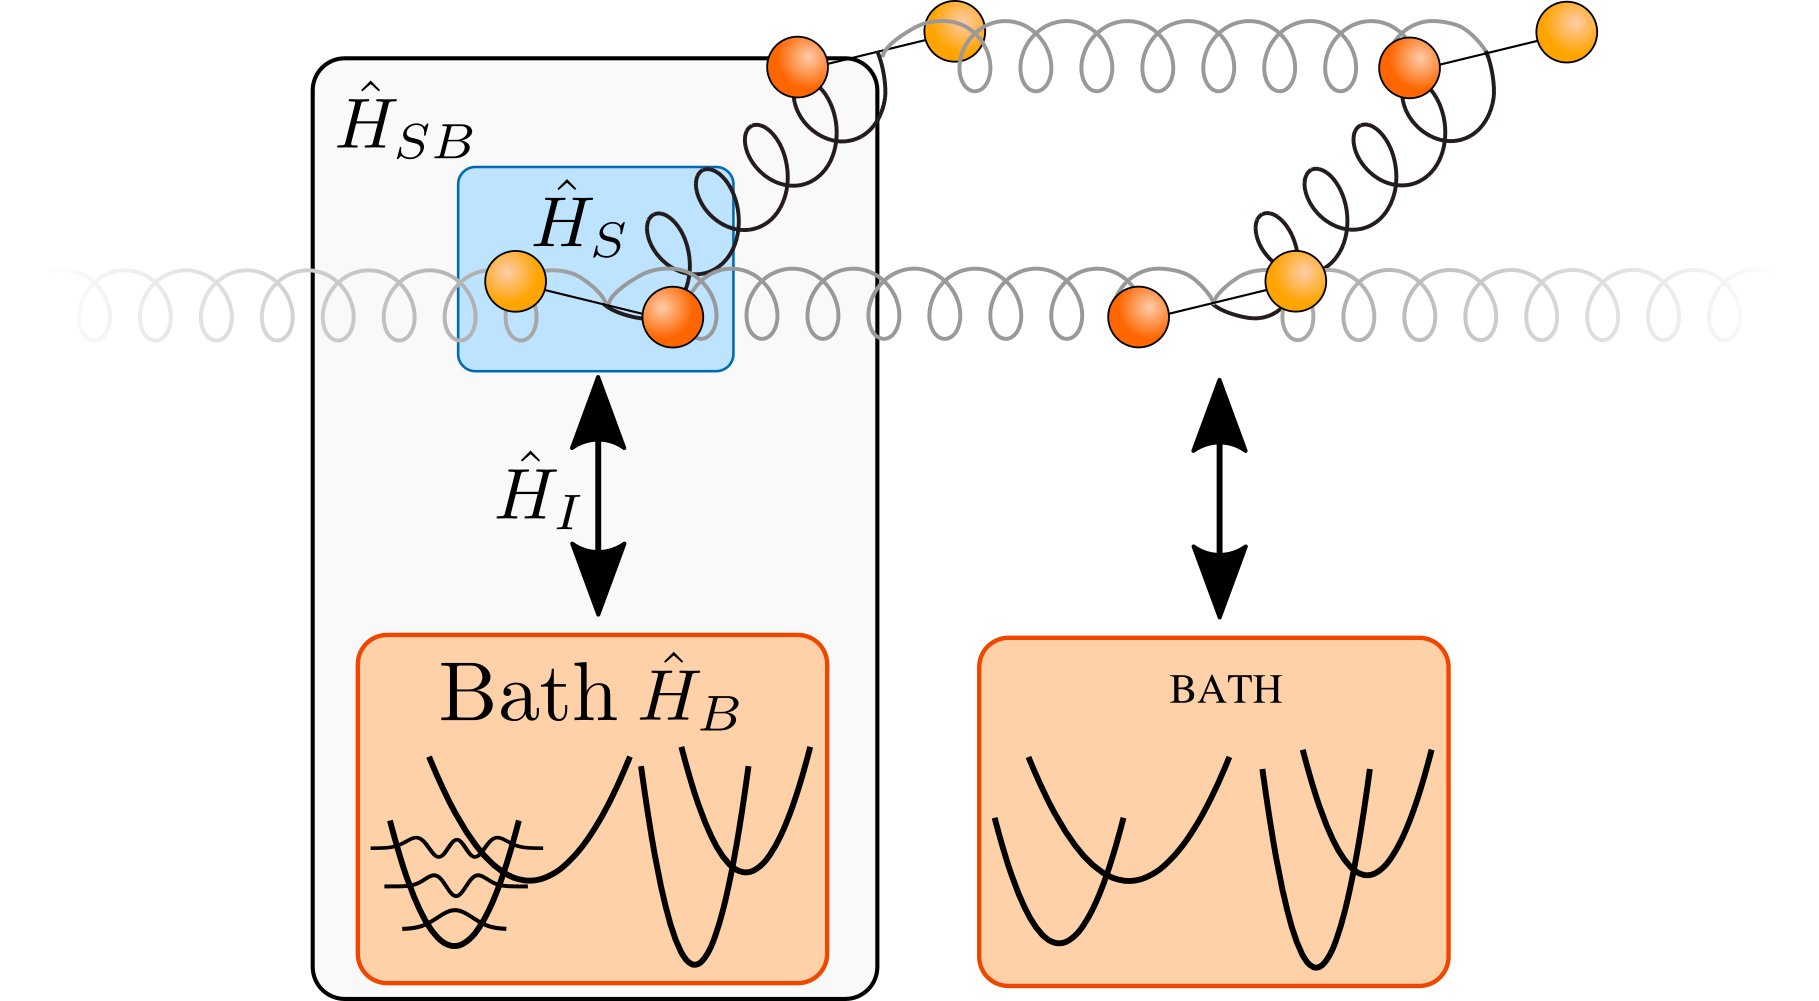
\includegraphics[width=0.8\linewidth]{graphics/OQS-Silicon.png}
		\caption{(CONCEPT) In the theory of open quantum systems, a system that is thermally coupled to an environment is modeled by a composite Hamiltonian $\hat{H}_{SB} =	\hat{H}_S + \hat{H}_B + \hat{H}_I$. $\hat{H}_S$ denotes the system Hamiltonian describing the potential acting on the dimer. The reservoir is modeled as a set of harmonic oscillators captured in $\hat{H}_B$. The interaction between a dimer and the bath are contained in $\hat{H}_I$. We approximate that every dimer is coupled to a separate bath.}
		\label{Figure::OQS-Silicon}
	\end{figure}
	To guarantee positivity of the $\hat{H}_{SB}$, a \textbf{counter-term}
	\begin{equation}
		\hat{H}_c =	\hat{x}^2 \sum_n \frac{\kappa_n^2}{2 m_n \omega_n^2} 
	\end{equation}
	is added. Positive Hamiltonians have solely positive eigenvalues, ensuring that the physical frequencies of motion of the Brownian particle are reproduced. In the following the counter-term is absorbed into $\hat{H}_S$. \\
	
	Since it is neither possible, nor required to solve the dynamics of the whole Hamiltonian, a probabilistic description will be developed. In quantum mechanics this is achieved by modeling the system density matrix $\hat{\rho}_{S}$. The density matrix of the composite system in \textbf{interaction picture} with respect to $\hat{H}_S + \hat{H}_B$ is given by
	\begin{equation}
		\boldsymbol{\hat{\rho}}_{SB} :=	e^{\mathrm{i} \left(\hat{H}_S + \hat{H}_B\right)t} \hat{\rho}_{SB} e^{-\mathrm{i} \left(\hat{H}_S + \hat{H}_B\right)t} ~.
	\end{equation}
	%Starting point is the von Neumann equation for $\boldsymbol{\hat{\rho}}_{SB} :=	e^{\mathrm{i} \left(\hat{H}_S + \hat{H}_B\right)t} \hat{\rho}_{SB} e^{-\mathrm{i} \left(\hat{H}_S + \hat{H}_B\right)t}$ in \textbf{interaction picture} with respect to $\hat{H}_S + \hat{H}_B$:
	Operators in interaction picture are printed \textbf{bold} in the following. The time evolution of $\boldsymbol{\hat{\rho}}_{SB}$ is
	\begin{equation} \label{Eq::OQS-Startpoint}
		\frac{\partial}{\partial t}\boldsymbol{\hat{\rho}}_{SB}(t) =	- \mathrm{i} \left[\boldsymbol{\hat{H}}_I(t), \boldsymbol{\hat{\rho}}_{SB}(t) \right] ~.
	\end{equation}
	To derive an equation for $\boldsymbol{\hat{\rho}}_S$ the reservoir degrees of freedom are traced out
	\begin{equation} \label{Eq::Tracing-Out-Reservoir}
		\begin{split}
			\frac{\partial}{\partial t} \boldsymbol{\hat{\rho}}_S(t) &=	\text{tr}_B \left \lbrace \frac{\partial}{\partial t} \boldsymbol{\hat{\rho}}_{SB}(t) \right \rbrace =	-\mathrm{i}~\text{tr}_B \left\lbrace \left[\boldsymbol{\hat{H}}_I(t), \boldsymbol{\hat{\rho}}_{SB}(t)\right] \right\rbrace  \\
			&=	-\mathrm{i}~\text{tr}_B \left\lbrace \left[\boldsymbol{\hat{H}}_I(t), \boldsymbol{\hat{\rho}}_{SB}(0)\right] \right \rbrace - \int_{0}^{t} \text{d}t'~ \text{tr}_B \left\{  \left[\boldsymbol{\hat{H}}_I(t), \left[\boldsymbol{\hat{H}}_I(t'), \boldsymbol{\hat{\rho}}_{SB}(t') \right]\right]  \right\} \\
			&=- \int_{0}^{t} \text{d}t'~ \text{tr}_B \left\{  \left[\boldsymbol{\hat{H}}_I(t), \left[\boldsymbol{\hat{H}}_I(t'), \boldsymbol{\hat{\rho}}_S(t') \otimes \overline{\rho}_B \right]\right]  \right\}~.
		\end{split}
	\end{equation}
	The second line in \autoref{Eq::Tracing-Out-Reservoir} is obtained by integrating \autoref{Eq::OQS-Startpoint} and solving for $\boldsymbol{\hat{\rho}}_{SB}(0)$. The \textbf{Born approximation}  assumes that the reservoir density matrix is stationary. In this case, the composite density matrix decomposes to $\boldsymbol{\hat{\rho}}_{SB}(t) = \boldsymbol{\hat{\rho}}_S(t) \otimes \overline{\rho}_B$ and the trace 
	\begin{equation}
		\text{tr}_B \left\lbrace \left[\boldsymbol{\hat{H}}_I(t), \boldsymbol{\hat{\rho}}_{SB}(0)\right] \right \rbrace =	0
	\end{equation}
	vanishes. The integrand in  \autoref{Eq::Tracing-Out-Reservoir} typically decays rather fast. Hence, the \textbf{Markov approximation} \cite{landi2022nonequilibrium} is applicable. This involves the replacement $\boldsymbol{\hat{\rho}}_S(t') \rightarrow \boldsymbol{\hat{\rho}}_S(t)$, as well as  sending the upper limit of the integral to infinity. Substituting $\tau =t - t'$ yields the \textbf{Redfield-II} master equation
	\begin{equation} \label{Eq::Redfield-II}
		\frac{\partial}{\partial t} \boldsymbol{\hat{\rho}}_S(t) = - \int_{0}^{\infty} \text{d}\tau~ \text{tr}_B \left\{  \left[\boldsymbol{\hat{H}}_I(t), \left[\boldsymbol{\hat{H}}_I(t - \tau), \boldsymbol{\hat{\rho}}_S(t) \otimes \overline{\rho}_B \right]\right]  \right\} ~.
	\end{equation}
	Transforming \autoref{Eq::Redfield-II} back to the Schrödinger picture gives
	\begin{equation} \label{Eq::Caldeira-Legget-Startpoint}
		\frac{\partial}{\partial t} {\hat{\rho}}_S(t) =	-\mathrm{i}~\left[\hat{H}_S, \rho_S(t)\right] - \int_{0}^{\infty} \text{d}\tau~ \text{tr}_B \left\{  \left[{\hat{H}}_I, \left[{\boldsymbol{\hat{H}}}_I(- \tau), {\hat{\rho}}_S(t) \otimes \overline{\rho}_B \right]\right]  \right\}~.
	\end{equation}
	The integral in the second term of \autoref{Eq::Caldeira-Legget-Startpoint} can be rearranged to
	\begin{equation} \label{Eq::CD-Trace-with-Kernels}
		\int_{0}^{\infty} \text{d}\tau \left(\frac{\mathrm{i}}{2} D(\tau) \left[\hat{x}, \left\{\boldsymbol{\hat{x}}(-\tau). \hat{\rho}_S(t)\right\}\right] - \frac{1}{2} D_1(\tau) \left[\hat{x}, \left[\boldsymbol{\hat{x}}(-\tau) , \hat{\rho}_S(t)\right]\right]\right)~,
	\end{equation}
	with the noise kernel $D_1(\tau)$ and dissipation kernel $D(\tau)$ defined as in \autoref{Section::Appendix-Caldeira-Legget}. The noise and dissipation kernels disappear on the timescale of the relaxation $\tau_B$ of the reservoir. When doing the Markov approximation it is assumed that this timescale is much shorter than the relaxation time of the system $\tau_S$. This is used again by approximating $\boldsymbol{\hat{x}}(-\tau)$ by its free dynamics
	\begin{equation}
		\boldsymbol{\hat{x}}(-\tau) =	\hat{x} - \hat{p} \tau~.
	\end{equation}
	Plugging this approximation into \autoref{Eq::CD-Trace-with-Kernels} allows for the evaluation of the integrals (see \autoref{Section::Appendix-Caldeira-Legget}). This eventually yields the \textbf{Caldeira-Leggett master equation}
	\begin{equation} \label{Eq::Caldeira-Leggett-Master-equation}
		\frac{\text{d}}{\text{d}t} \rho_S(t) =	\underbrace{-\mathrm{i}\left[\hat{H}_S, \rho_S(t) \right]}_{\text{free dynamics}} - \underbrace{\mathrm{i} \eta \Big [\hat{x}, \big\{\hat{p}, \rho_S(t)\big\}\Big ]}_\text{dissipative term} - \underbrace{2 \eta m k_B T \Big [\hat{x}, \big[\hat{x}, \rho_S(t)\big]\Big ]}_\text{thermal fluctuations}~.
	\end{equation}
	The damping constant $\eta$ enters the calculation through a parametrization of the spectral density function of the reservoir. The first term in the Caldeira-Leggett master equation describes the free dynamics of the system and resembles the form of the \textbf{von-Neumann} equation. The second term is the dissipative part proportional to the damping constant $\eta$. The thermal fluctuations of the reservoir are captured in the third term proportional to the temperature $T$. The state of the reservoir $\overline{\rho}_B$ follows the \textbf{Bose-Einstein distribution} and determines $T$.
	\subsection{Equations of Motion}
	From \autoref{Eq::Caldeira-Leggett-Master-equation} one can derive equations of motion for arbitrary observables via
	\begin{equation}\label{Eq::QM-Eq-of-motion}
		\frac{\text{d}}{\text{d}t} \left \langle \hat{A} \right \rangle =	\text{tr} \left\{\hat{A} \frac{\text{d}}{\text{d}t } \hat{\rho}_S(t)\right\}~.
	\end{equation}
	\textcolor{red}{Version 1:}
	Comparing the results of \autoref{Eq::QM-Eq-of-motion} for $\hat{x}, \hat{p}$ and $\hat{p}^2$ to the equations of Brownian motion of \autoref{Section::Brownian-Motion}
	\begin{multicols}{2}
		\noindent
		\begin{align*}
			\begin{split}
				&\frac{\text{d}}{\text{d}t} \left \langle \hat{x} \right \rangle =	\frac{1}{m} \left\langle \hat{p} \right \rangle~,
			\end{split}
			\\
			\begin{split}
				&\frac{\text{d}}{\text{d}t} \left \langle \hat{p} \right \rangle = - 	\left\langle  \frac{\partial V(\hat{x})}{\partial \hat{x}} \right \rangle - \eta \left \langle \hat{p} \right \rangle ~,
			\end{split}
			\\
			\begin{split}
				&\frac{\text{d}}{\text{d}t} \left \langle \hat{p}^2 \right \rangle =	- \left\langle \hat{p} \frac{\partial V(\hat{x})}{\partial \hat{x}} + \frac{\partial V(\hat{x})}{\partial \hat{x}} \hat{p} \right \rangle \\
				&\qquad \qquad ~- 2 \eta \left \langle \hat{p}^2 \right \rangle + 2 \eta k_B T ~,
			\end{split}
		\end{align*}
		\begin{align*}
			\begin{split}
				&\frac{\text{d}}{\text{d}t} \left \langle {x}(t) \right \rangle  =	~\frac{1}{m} \left \langle {p}(t) \right \rangle ~,
			\end{split}
			\\
			\begin{split}
				&\frac{\text{d}}{\text{d}t} \left \langle {p}(t) \right \rangle =	- 	\left \langle \frac{\partial V({x})}{\partial {x}} \right \rangle - \eta \left \langle {p}(t) \right \rangle ~,
			\end{split}
			\\
			\begin{split}
				&\frac{\text{d}}{\text{d}t} \left \langle {p}^2(t) \right \rangle = - \left\langle 2 {p}(t) \frac{\partial V({x})}{\partial {x}}\right \rangle \\
				&\qquad \qquad \quad ~ - 2 \eta \left \langle {p}^2(t) \right \rangle + 2 \eta k_B T~.
			\end{split}
		\end{align*}
	\end{multicols}	
	\begin{table}[h]
		\centering
		\caption{Version2.1.The equations of motion for  $\hat{x}, \hat{p}$ and $\hat{p}^2$ calculated from  \autoref{Eq::QM-Eq-of-motion} are compared to Brownian motion of \autoref{Section::Brownian-Motion}. It is evident that the structure of equations of motion for the quantum expectation values matches the expectation values from Brownian motion. Therefore the quantum mechanical case is called \textbf{Quantum Brownian Motion}.}
		\begin{tabular}{l l}
			\toprule
			Quantum Brownian Motion  & $\quad$ $\quad$ \\
			\midrule
			Eq. for $\left \langle \hat{x} \right \rangle$: & $\frac{\text{d}}{\text{d}t} \left \langle \hat{x} \right \rangle =	\frac{1}{m} \left\langle \hat{p} \right \rangle$ \\
			Eq. for $\left \langle \hat{p} \right \rangle$: & $\frac{\text{d}}{\text{d}t} \left \langle \hat{p} \right \rangle = - 	\left\langle  \frac{\partial V(\hat{x})}{\partial \hat{x}} \right \rangle - \eta \left \langle \hat{p} \right \rangle$ \\
			Eq. for $\left \langle \hat{p}^2 \right \rangle$: & $\frac{\text{d}}{\text{d}t} \left \langle \hat{p}^2 \right \rangle =	- \left\langle \hat{p} \frac{\partial V(\hat{x})}{\partial \hat{x}} + \frac{\partial V(\hat{x})}{\partial \hat{x}} \hat{p} \right \rangle- 2 \eta \left \langle \hat{p}^2 \right \rangle + 2 \eta k_B T$  \\
			\midrule
			Brownian Motion  & $\quad$ $\quad$ \\
			\midrule
			Eq. for $\left \langle {x}(t) \right \rangle$: & $\frac{\text{d}}{\text{d}t} \left \langle {x}(t) \right \rangle  =	~\frac{1}{m} \langle {p}(t) \rangle $ \\
			Eq. for $\left \langle {p}(t) \right \rangle$: & $\frac{\text{d}}{\text{d}t} \left \langle {p}(t) \right \rangle =	- 	\left \langle \frac{\partial V({x})}{\partial {x}} \right \rangle - \eta \left \langle {p}(t) \right \rangle$ \\
			Eq. for $\left \langle {p}^2(t) \right \rangle$: & $\frac{\text{d}}{\text{d}t} \left \langle {p}^2(t) \right \rangle = - \left\langle 2 {p}(t) \frac{\partial V({x})}{\partial {x}}\right \rangle - 2 \eta \left \langle {p}^2(t) \right \rangle + 2 \eta k_B T$   \\
			\bottomrule
		\end{tabular}
		\label{Table::QBM-vs-BM}
	\end{table}
	\begin{table}[h]
		\centering
		\caption{Version2.2. The equations of motion for  $\hat{x}, \hat{p}$ and $\hat{p}^2$ calculated from  \autoref{Eq::QM-Eq-of-motion} are compared to Brownian motion of \autoref{Section::Brownian-Motion}. It is evident that the structure of equations of motion for the quantum expectation values matches the expectation values from Brownian motion. Therefore the quantum mechanical case is called \textbf{Quantum Brownian Motion}.}
		\renewcommand{\arraystretch}{1.7}
		\begin{tabular}{c l l}
			\toprule
			Quantity & Quantum Brownian Motion $\qquad$  & Brownian Motion \\
			\midrule
			$x$ & $\frac{\text{d}}{\text{d}t} \left \langle \hat{x} \right \rangle \hspace{3pt}=	\frac{1}{m} \left\langle \hat{p} \right \rangle$ & $\frac{\text{d}}{\text{d}t} \left \langle {x}(t) \right \rangle \hspace{3pt}  =	~\frac{1}{m} \langle {p}(t) \rangle $ \\
			$p$ & $\frac{\text{d}}{\text{d}t} \left \langle \hat{p} \right \rangle ~= - 	\left\langle  \frac{\partial V(\hat{x})}{\partial \hat{x}} \right \rangle - \eta \left \langle \hat{p} \right \rangle$ &	$\frac{\text{d}}{\text{d}t} \left \langle {p}(t) \right \rangle ~=	- 	\left \langle \frac{\partial V({x})}{\partial {x}} \right \rangle - \eta \left \langle {p}(t) \right \rangle$ \\
			$p^2$ & \makecell[l]{$\frac{\text{d}}{\text{d}t} \left \langle \hat{p}^2 \right \rangle =	- \left\langle \hat{p} \frac{\partial V(\hat{x})}{\partial \hat{x}} + \frac{\partial V(\hat{x})}{\partial \hat{x}} \hat{p} \right \rangle$ \\ $ \qquad \qquad \hspace{2pt} - 2 \eta \left \langle {p}^2(t) \right \rangle + 2 \eta k_B T$} & \makecell[l]{$\frac{\text{d}}{\text{d}t} \left \langle {p}^2(t) \right \rangle = - \left\langle 2 {p}(t) \frac{\partial V({x})}{\partial {x}}\right \rangle $ \\ $ \qquad \qquad \hspace{3pt} \quad - 2 \eta \left \langle {p}^2(t) \right \rangle + 2 \eta k_B T$}\\
			\bottomrule
		\end{tabular}
		\label{Table::QBM-vs-BM}
	\end{table} \renewcommand{\arraystretch}{1.2}
	shows that the two equation sets share the same structure.\\
	\textcolor{red}{Version 2:}\\
	The results of \autoref{Eq::QM-Eq-of-motion} for $\hat{x}, \hat{p}$ and $\hat{p}^2$ are compared to the equations of Brownian motion of \autoref{Section::Brownian-Motion} in \autoref{Table::QBM-vs-BM}. The two equation sets share the same structure. \\
	
	Especially interesting is the last term in the equations for $\langle \hat{p}^2 \rangle$. This is the diffusion constant in the case of Brownian motion and it matches the quantum mechanical term. Hence, it is possible to derive the diffusion constant from microscopic considerations. We conclude that the classical equations of motion \autoref{Eq::Langevin-eq-motion-set-x} and \autoref{Eq::Langevin-eq-motion-set-p} are the classical correspondence to the equations of $\langle \hat{x} \rangle$ and $\langle \hat{p} \rangle$. In the following, the classical equations of motion will be used to describe the silicon surface. Since the silicon dimers interact, the potential $V(x) =	V(x, {x_i})$ is a function of the coordinates $x_i$ of the other dimers, leading to a \textbf{coupling} between the differential equations. Additionally, $V(x, {x_i})$ is \textbf{nonlinear} in $x$, eventually yielding a coupled set of nonlinear stochastic differential equations. An analytic solution is impossible and therefore we turn to numerical solutions in the next section.
	\section{Numerical Methods and Molecular Dynamics} \label{Section::Numerical-methods}
	The update-form \autoref{Eq::std-langevin-eq} of the Langevin equation is very useful for its numerical solution. A simple method of solution is the straight implementation of \autoref{Eq::std-langevin-eq}, which is called the \textbf{Euler-Maruyama method} \cite{kloeden1992stochastic}. Practically, a system of first-order stochastic differential equations
	\begin{align}
		&x(t + \text{d}t) = x(t)	+ \frac{1}{m} p(t) \text{d}t ~, \\
		&p(t + \text{d}t) =	p(t) - \frac{\eta}{m} p(t) \text{d}t - \frac{\partial V(x(t))}{\partial x} \text{d}t + \sqrt{2 k_B T \eta} ~ n(t) \sqrt{\text{d}t} ~,
	\end{align}
	is solved. The Euler-Maruyama method is straightforward to implement and computationally inexpensive, but shows discretization artefacts even for small stepsizes $\text{d}t$. Since the integration of the equations of motion usually takes much less time than the evaluation of $V(x(t))$ \cite{frenkel2023understanding}, many efforts have been made to improve the weak convergence \cite{kloeden1992stochastic} of integration schemes. \\
	
	The topic of simulating microscopical systems by numerically solving Newton's equations of motion is called \textbf{molecular dynamics}. Molecular dynamics is widely used in biophysics, chemical physics but also material sciences. Larini et al. \cite{larini2007langevin} compare some of the integration schemes that have been developed. They show that the popular Brunger-Brooks-Karplus (BBK) \cite{brunger1984stochastic} scheme is robust method with a number of general advantages. It integrates in three steps \cite{izaguirre2001langevin}, half a kick
	\begin{equation}
		p\left(t + \tfrac{1}{2} \text{d}t \right) =	\left(1 - \tfrac{1}{2} \eta \text{d}t \right) p(t) - \tfrac{1}{2} \text{d}t \tfrac{\partial V(x(t))}{\partial x} + \tfrac{1}{2} \sqrt{2\eta{k_B T}} n(t) \sqrt{\text{d}t}~,
	\end{equation}
	drift
	\begin{equation}
		x(t + \text{d}t) = x(t) +  p\left(t + \tfrac{1}{2} \text{d}t\right) \text{d}t~,
	\end{equation}
	and half a kick
	\begin{equation}
		p\left(t\right) =	\left(1 + \tfrac{\text{d}t}{2} \eta \right)^{-1} \left( p\left(t + \tfrac{\text{d}t}{2}\right) - \tfrac{1}{2} \text{d}t \tfrac{\partial V(x(t + \text{d}t))}{\partial x} + \tfrac{1}{2} \sqrt{2\eta{k_B T}} n({t + \text{d}t}) \sqrt{\text{d}t} \right) ~.
	\end{equation}
	%	\begin{align}
		% 		\nonumber \\
		%		&p_i\left(t + \tfrac{1}{2} dt \right) =	\left(1 - \tfrac{1}{2} \eta dt \right) p_i(t) - \tfrac{1}{2} dt \tfrac{\partial V(x_i(t), \{x\})}{\partial x_i} + \tfrac{1}{2} \sqrt{2\eta{k_B T}} n_i(t) \sqrt{dt}~, \nonumber \\
		%		&\text{drift} \nonumber \\
		%		&x_i(t + dt) = x_i(t) +  p_i\left(t + \tfrac{1}{2} dt\right) dt~, 		\label{Eq::BBK-method} \\
		%		&\text{half a kick} \nonumber \\
		%		&p_i\left(t\right) =	\left(1 + \tfrac{dt}{2} \eta \right)^{-1} \left( p_i\left(t + \tfrac{dt}{2}\right) - \tfrac{1}{2} dt \tfrac{\partial V(x_i(t + dt), \{x\})}{\partial x_i} + \tfrac{1}{2} \sqrt{2\eta{k_B T}} n_i({t + dt}) \sqrt{dt} \right)\nonumber.
		%	\end{align}
	Compared to higher-order schemes, like the fourth-order Hamiltonian Runge-Kutta scheme \cite{press2002numerical}, that require multiple potential evaluations, the BBK method is faster with limited loss of accuracy \cite{larini2007langevin}. The BBK integration step is slightly slower than the Euler-Maruyama one but it makes up through its much greater stability regarding larger step sizes. This ultimately results in significantly faster simulation speeds. The stability of the schemes is compared in \autoref{Section::Benchmarks}. \\
	
	The theoretical foundation for the simulation of the Si(001) surface using Langevin equations is now established. The following section will deal with the modeling of the several times mentioned potential.
	\section{The Model}
	\subsection{The Ising model}
	The Ising model is well known and has been used several times \cite{brand2023dimer, pillay2004revisit, ihm1983structural, schaller2023sequential} to study the Si(001) surface. Brand et al. \cite{brand2023critical} found good agreement between the Si(001) phase transition and the Ising critical exponents.  Their results are relevant for the following investigations and therefore the Ising model will be shortly discussed below. \\
	
	The two-dimensional Ising model describes spins $\sigma_{i ,j} =	\pm 1$ on a lattice. Consider the anisotropic case on a rectangle without external field. Its nearest-neighbor Hamiltonian is given by
	\begin{equation} \label{Eq::Ising-Hamiltonian}
		H =	- \sum_{i,j}^{} \left(J_\parallel \sigma_{i ,j} \sigma_{i ,j + 1} + J_\perp \sigma_{i, j} \sigma_{i +1 ,j} \right) ~,
	\end{equation}
	with $J_{\delta}$, $\delta \in \{\parallel, \perp\}$, being the effective nearest-neighbor coupling strengths. The two-dimensional anisotropic Ising model is analytically solvable \cite{onsager1944crystal} and exhibits a continuous phase transition at
	\begin{equation} \label{Eq::Crit-Temp-Ising}
		\sinh \left( \frac{2 |J_\parallel|}{k_B T_c} \right) \sinh \left( \frac{2 |J_\perp|}{k_B T_c}\right) =	1.
	\end{equation}
	The equilibrium correlation lengths for $T > T_c$ can be determined from the coupling constants \cite{mccoy1973two} by
	\begin{equation} \label{Eq::Ising-Corrlength-Coupling}
		\frac{\xi_\delta(T_c)}{a_\delta} =	\left(\ln \left[ \coth \left(\frac{|J_\delta|}{k_B T_c}\right)\right] - \frac{2 |J_{\overline{\delta}}|}{k_B T}\right)^{-1} ~,
	\end{equation}
	with $a_\delta$ being the lattice spacing in $\delta$ direction and $\overline{\delta}$ marking the direction perpendicular to $\delta$. \\
	
	To describe the silicon surface with the Ising model, the equilibrium positions of the silicon dimers in \autoref{Fig::dimer-configs} (b) are mapped to the Ising spin values $\sigma_{i ,j} =	\pm 1$. In theoretical works, density functional theory (DFT) calculations are often employed to calculate configuration energies.   \autoref{Eq::Ising-Hamiltonian} can then be used to fit effective  $J_\delta$ to the DFT results. In experiments, the correlation lengths $\xi_\delta$ can be measured and used to extract $J_\delta$ through \autoref{Eq::Ising-Corrlength-Coupling}. Calculating quantitative values for $J_\delta$ can reveal important information about the nature of the microscopic interactions (between the dimers), especially if \autoref{Eq::Ising-Hamiltonian} is extended to next-nearest neighbor couplings or even further. Additionally, theoretical
	\begin{wrapfigure}[17]{r}{0.35\textwidth}
		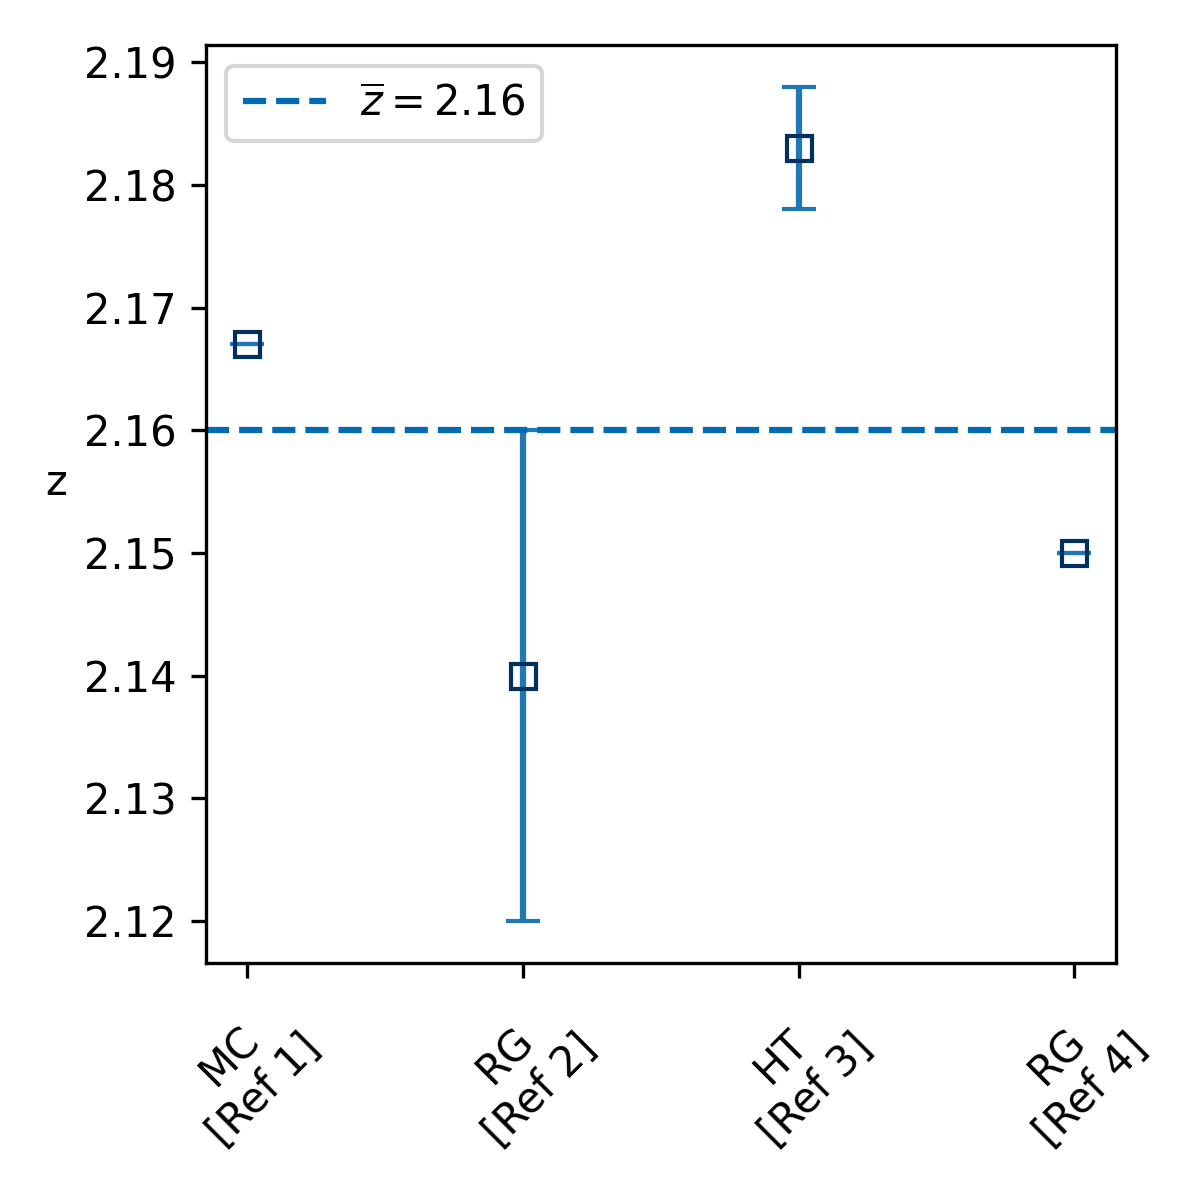
\includegraphics[width=\linewidth]{graphics/z-values}
		\caption{Recent results for the dynamic critical exponent $z$ are summarized. The datapoints are obtained by Monte-Carlo methods (MC) \cite{nightingale2000monte}, renormalization group calculations (RG) \cite{adzhemyan2022dynamic, duclut2017frequency} and high-temperature expansion (HT) \cite{dammann1993dynamical}.}
		\label{Figure::Ising-z-values}
	\end{wrapfigure}
	results of the Ising model can be used to analyze the surface further. For example, \autoref{Eq::Crit-Temp-Ising} may be used to estimate the transition temperature. Eventually, a simple theoretical model of the Si(001) system is obtained which also may be used in computer simulations.\\
	
	The Ising model gives name to its universality class. It is characterized by a continuous phase transition with a scalar order parameter and $\mathbb{Z}_2$ symmetry. The static critical exponents of the Ising universality class can be calculated analytically \cite{cardy1996scaling}. For $\nu$ the exact value
	\begin{equation}
		\nu =	1
	\end{equation}
	is obtained. As noted in \autoref{Section::Dynamic-Scaling}, the anisotropic Ising model is part of Model A of critical dynamics \cite{hohenberg1977theory}. The constant $c$ of \autoref{Eq::Model-A-z} has been estimated by numerous method. Some recent results for $z$ are shown in \autoref{Figure::Ising-z-values}. \\
	%An overview of the relevant critical exponents is given in \autoref{Table::Ising-crit-expo}.
	
	Since the Ising model has discrete states, it is not suitable for continuous modeling with equations of motion.
	%	\begin{table}[hb]
		%		\centering
		%		\begin{tabular}{c c c}
			%			$\qquad \nu \qquad$ & z & $ \quad ~ \tfrac{\nu}{1 + \nu z} ~ \quad$ \\
			%			1 & $2.1667 \pm 0.0005$ & $0.3158 \pm ?$ \\
			%		\end{tabular}
		%		\caption{The static critical exponents of the Ising universality class can be calculated analytically \cite{cardy1996scaling}. The value for $z$ is the estimate of Nightingale et al. \cite{nightingale2000monte}, who used MC techniques.}
		%		\label{Table::Ising-crit-expo}
		%	\end{table}
	\subsection{The Classical XY Model}
	The classical XY model and the Ising model can be viewed as two special cases of the Potts model \cite{potts1952some}. It generalizes the Ising model to allow $q$, instead of two, states. The states are uniformly distributed on a circle as shown in \autoref{Fig::States} (a). In the limit $q \rightarrow \infty$ the XY model is obtained. It allows continuous states on the unit circle and is thus suitable to be described by Langevin equations. \\
	
	The two-dimensional XY Hamiltonian with nearest-neighbor interactions is given by
	\begin{equation}
		\begin{split}
			H =&- \sum_{i,j}^{} \left(J_\parallel \vec{s}_{i,j} \vec{s}_{i,j + 1} + J_\perp  \vec{s}_{i,j} \vec{s}_{i + 1,j} \right)   \\
			=&- \sum_{i,j}^{} \left(J_\parallel  \cos \left(\vartheta_{i,j} - \vartheta_{i, j+1} \right) + J_\perp  \cos \left(\vartheta_{i,j} - \vartheta_{i+1, j} \right) \right)	 ~,
		\end{split}
	\end{equation}
	with unit-length vectors
	\begin{equation}
		\vec{s}_{i, j} =	\left(\begin{array}{c}
			\cos \vartheta_{i, j} \\
			\sin \vartheta_{i, j}
		\end{array}\right) ~,
	\end{equation}
	characterizing the state of the lattice site. These rotors are defined by a continuous angle $\vartheta$ on the interval $[0, 2\pi)$. Although the exact solution of the two-dimensional XY model is intractable, Mattis \cite{mattis1984transfer} used a transfer matrix approach to approximate an analogue to \autoref{Eq::Crit-Temp-Ising}. He arrived at
	\begin{equation} \label{Eq::Crit-Temp-XY}
		\frac{2 k_B T_c}{J_\parallel} \ln \left(\frac{2 k_B T_c}{J_\perp}\right) =	1 ~, 
	\end{equation}
	with $J_\parallel \geq J_\perp$. The relation between the coupling constants and the equilibrium correlation lengths is not known at the moment. \\
	
	The two-dimensional XY model does not exhibit a phase transition in the conventional sense. The \textbf{Mermin-Wagner theorem} \cite{mermin1966absence} prohibits the breaking of its continuous $\text{O}(2)$ symmetry through short-range interactions. Instead, the system shows the \textbf{Kosterlitz-Thouless transition} (KT transition) \cite{JMKosterlitz_1973, berezinskii1971destruction}. The usual power laws are not applicable to this transition because the correlation length diverges exponentially at the critical point. Hence, the two-dimensional XY model does not belong to any universality class. \\
	
	We can add a $p$-fold symmetry breaking field of strength $h$ to the XY Hamiltonian
	\begin{equation} \label{Eq::XY-Hamilton-Field}
		H =- \sum_{i,j}^{} \left(J_\parallel  \cos \left(\vartheta_{i,j} - \vartheta_{i, j+1} \right) + J_\perp  \cos \left(\vartheta_{i,j} - \vartheta_{i+1, j} \right) \right)	+ h \sum_{i,j} \cos(p\vartheta_{i,j}) ~,
	\end{equation}
	explicitly breaking the $\text{O}(2)$ symmetry. Such fields may very well be experimentally realized by crystalline anisotropies. The Migdal lattice recursion scheme \cite{migdal1975phase} implies that for $T \rightarrow 0$, the field $h$ is a relevant variable in the sense of \autoref{Section::RG}. The perturbations caused by $h$ will grow as $T$ shrinks, eventually forcing the system into a state of broken symmetry in which one of the directions $\vartheta =	{2 \pi n }/{p}, n \in \left[0, p-1\right]$ is preferred. Hence, any $h$ will lead to deviations in critical behavior from the KT transition. José and Kadanoff \cite{jose1977renormalization} found that this symmetry broken XY model exhibits a continuous phase transition with the critical exponents of a $p$-state Potts model. This results in Ising critical behavior in the case of $p=2$. This makes the two-dimensional XY model with twofold symmetry breaking field ideal to explore the dynamics of the Si(001) surface.
	\begin{figure}[htp]
		\centering
		\begin{subfigure}{\textwidth}
			\centering
			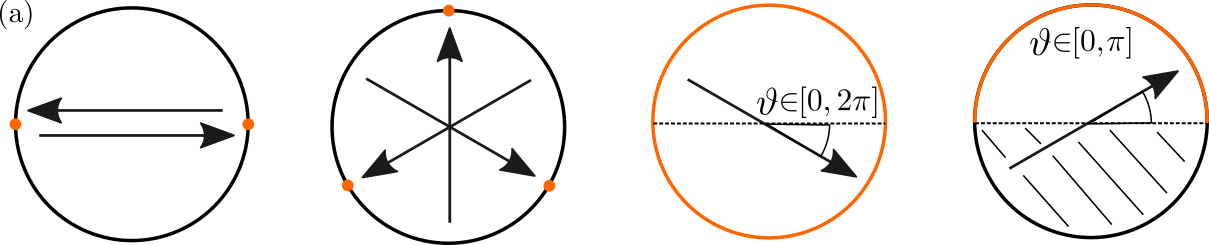
\includegraphics[width=0.9\linewidth]{graphics/Allowed-States.png}
		\end{subfigure} \\
		\par\bigskip % force a bit of vertical whitespace
		\begin{subfigure}{\textwidth}
			\centering
			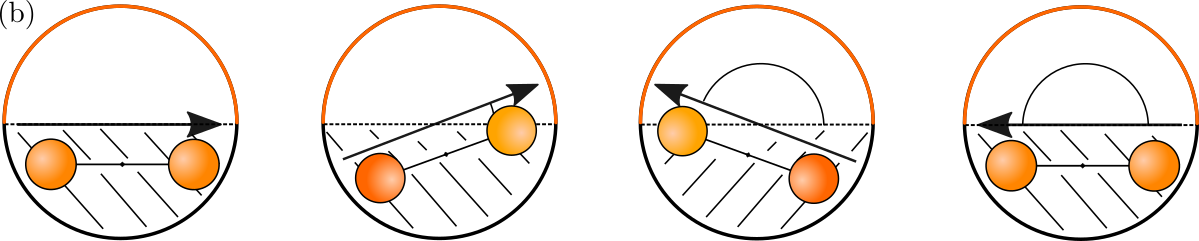
\includegraphics[width=0.9\linewidth]{graphics/State-Mapping.png}
		\end{subfigure}
		\caption{Unit circles are shown as visualizations of the state space. The orange parts are the allowed states. The states are depicted as arrows inside the unit circle. \textbf{(a)} shows the $q$-state Potts model. From left to right: The two-state Potts model, or the Ising model, allows only two points on the unit circle.  The three-state Potts model allows three different spin directions, visualized by the arrows. In the limit $q \rightarrow \infty$ the XY model is obtained. The state is characterized by a continuous angle $\vartheta$. The rightmost circle visualized the adaptation of the XY model to the silicon surface. Here, only half the circle is allowed. \textbf{(b)} The buckling angles of the silicon dimers are mapped to the rotors of the XY model. Since the silicon atoms are indistinguishable, a rotation by $\pi$ maps to the same state. Hence, the state space is only half the unit circle. Note that the left and right vectors are the same state and strictly speaking one of them can be excluded by defining $\vartheta \in [0, \pi)$.}
		\label{Fig::States}
	\end{figure}
	\subsection{Adaptation to the Si(001) Surface}\label{Sec::XY-to-Silicon}	
	In the following the XY model will be adapted to optimally resemble the silicon surface. \\ 	%In the following some customization steps will be shown to adapt the XY model in a way to optimally resemble the experimentally observed properties of the silicon surface. 
	
	Like done with the Ising model, the aim is to map the position of the dimer to a model state. The natural choice is to identify the dimer buckling angle with the rotor angle $\vartheta$ of the XY model. Since the silicon atoms are indistinguishable, a rotation by $\pi$ translates into the same state. Hence, only $\vartheta \in [0, \pi)$ define unique states, restricting the state space of the XY model. The resulting half circle is shown in the rightmost picture of \autoref{Fig::States} (a). For computational reasons, $\vartheta $ will be shifted by $-\tfrac{\pi}{2}$, eventually yielding $\vartheta \in \left[-\tfrac{\pi}{2}, \tfrac{\pi}{2}\right)$. The restriction is achieved by adding a factor $m=2$ into the interaction terms 
	\begin{equation}
		J_\delta \cos \left(m \Delta \vartheta_{i, j}\right)~.
	\end{equation}
	The equilibrium position of the dimers is majorly influenced by the location of the minima of the symmetry breaking field. The experimental systems shows two stable buckling angles of about $\pm 20^\circ$. Therefore the symmetry breaking field will be constructed to have two minima on the interval $\left[-\tfrac{\pi}{2}, \tfrac{\pi}{2}\right)$ at the desired angles. The minima satisfy
	%Since the silicon dimers do not have a distinguished direction in contrary to the spin vectors of the XY model, we define the right dimer to point along the arrow \autoref{Fig::DimerMapping}. Additionally, a flip of the pointer by $\pm \pi$ results in the same state, effectively cutting the state space in half. Measuring from the (001) axis (\autoref{Fig::SiliconDiamond}), the angles will be restricted to $\vartheta \in \left[-\tfrac{\pi}{2}, \tfrac{\pi}{2}\right]$.	This is achieved by adding a factor $m = 2$ into the $J_\delta \cos \left(m \Delta \vartheta_{i, j}\right)$ terms. As stated in \autoref{Section::Silicon}, the dimers are buckled by  $18^{\circ}$ corresponding to a an angle $\vartheta^\pm=	\pm 72^\circ \approx	\pm \tfrac{2}{5} \pi $~. The equilibrium positions of \autoref{Eq::XY-Hamilton-Field} are determined by the symmetry breaking field and the parameter $p$ since the interaction is $O(2)$-symmetric. The minima satisfy
	\begin{equation}
		\cos \left(p \vartheta^\pm\right) =	-1~,
	\end{equation}
	implying that roughly $ p \approx 2.5$. The final resting position of the dimer is shifted by the repulsive interaction of the dimers. This is covered in \autoref{Section::quantitative}. The movement of the dimers can be approximated to take place in a double well potential \cite{dabrowski1992self}. This is realized by the symmetry breaking shown in \autoref{Fig::XY-Silicon-Potential}. The question arises if the system still belongs to the Ising universality class if $p$ is a rational number and the allowed states are restricted. This will be subject of \autoref{Section::static-scaling}. \\
	
	%to ensure to reproduce the experimental equilibrium positions. The resulting potential of the symmetry breaking field is shown in \autoref{Fig::XY-Silicon-Potential}. \\
	\begin{figure}[thb]
		\centering
		\includegraphics[width=0.8\linewidth]{graphics/XY-Silicon-potential2.png}
		%\caption{The external field in combination with the restriction of $\vartheta$ leads to  the shown potential. The angle is measured from the $(110)$ axis for illustration purposes. The Dynamics of the dimers for sufficiently low temperatures will take place around $\vartheta =	0$, the bucklings of $\vartheta =	\pm \tfrac{1}{2} \pi$ will almost never be reached.}
		\caption{The symmetry breaking field $h$ is shown in blue on the dimer angle. The dimer states are defined on $\vartheta \in [-\tfrac{\pi}{2}, \tfrac{\pi}{2}]$, therefore $h$ repeats after a period of $\pi$. The location of the potential minima are chosen to be located at the according position of the experimental dimers. The red area around $\vartheta =	0$, corresponding to vertical dimers, is strongly suppressed and rarely realized. The dynamics take place in the double well potential shown on the left and on the right of the plot. Some dimer states are depicted at their according angle.}
		\label{Fig::XY-Silicon-Potential}
	\end{figure}
	A suitable order parameter for this model is
	\begin{equation} \label{Eq::Si-Order-Param}
		M_L =	\frac{1}{L^2} \sum_{i,j} m(\vartheta_{i, j}) \qquad \text{with} \qquad	m(\vartheta) =	\sin \left(\tfrac{p}{2} \vartheta\right) ~,
	\end{equation}
	as the $m(\vartheta)$ have maxima at $\vartheta^{+}$ and minima at $\vartheta^{-}$, satisfying $m(\vartheta^+) =	- m (\vartheta^-)$.
	
	The XY model's natural conjugated coordinate is the angle $\vartheta$ and therefore \autoref{Eq::Langevin-eq-motion-set-x} and \autoref{Eq::Langevin-eq-motion-set-p} have to be adapted to rotary motion. The velocity is replaced by the angular velocity $\omega$ in this case.
	
	\autoref{Eq::XY-Hamilton-Field} yields the force
	\begin{equation} \label{Eq::Potential-Derivative}
		\begin{split}
			\frac{\partial V(\{\vartheta\})}{\partial \vartheta_{i, j}} = ~~~& J_\parallel m \Big( \sin \left(\vartheta_{i,j} - \vartheta_{i + 1, j} \right) +   \sin \left(\vartheta_{i,j} - \vartheta_{i-1, j} \right) \Big)	 \\
			+ &J_\perp m \Big( \sin \left(\vartheta_{i,j} - \vartheta_{i, j+1} \right) +  \sin \left(\vartheta_{i,j} - \vartheta_{i, j-1} \right) \Big) \\
			+ &h p \sin(p\vartheta_i)~.
		\end{split}
	\end{equation}
	Eventually, the Langevin equations become
	\begin{align}
		&\frac{\text{d}}{\text{d}t} \vartheta_{i,j}(t) =	 \omega_{i,j}(t)~, \label{Eq::Si-Langevin-theta} \\
		&\frac{\text{d}}{\text{d}t} \omega_{i,j}(t) =	- \frac{\eta}{I} \omega_{i,j}(t) - \frac{1}{I}\frac{\partial V(\{\vartheta\})}{\partial \vartheta_{i,j}} + \sqrt{\frac{2 k_B T \eta}{I^2}} \Gamma(t)~, \label{Eq::Si-Langevin-omega}
	\end{align}
	with the moment of inertia $I$ replacing the mass $m$. The implementation of the integration of this coupled set of stochastic differential equations will be the subject of the next section.
	%	\begin{equation}
		%		\ddot{\vartheta}_{i, j} =	- \frac{\eta}{I} \dot{\vartheta}_{i, j} - \frac{1}{I} V_{i,j}' + \sqrt{\frac{2 k_B T \eta}{I^2}} \Gamma_{i,j}
		%	\end{equation}
	
	
	\appendix
	\chapter{Appendix}
	\section{Caldeira-Legget calculation} \label{Section::Appendix-Caldeira-Legget}
	Starting point for this calculation is \autoref{Eq::Caldeira-Legget-Startpoint}. Consider the trace in the second term in \autoref{Eq::Caldeira-Legget-Startpoint}:
	\begin{equation}
		\text{tr}_B \left\{  \left[{\hat{H}}_I, \left[{\boldsymbol{\hat{H}}}_I(- \tau), {\hat{\rho}}_S(t) \otimes \overline{\rho}_B \right]\right]  \right\} =	\text{tr}_B \left\{  \left[\hat{x} \otimes \hat{B}, \left[{\boldsymbol{\hat{x}}}(- \tau) \otimes \boldsymbol{\hat{B}}(- \tau), {\hat{\rho}}_S(t) \otimes \overline{\rho}_B \right]\right]  \right\}~.
	\end{equation}
	Multiplying out the commutator yields
	\begin{equation} \label{Eq::Caldeira-Leggett-Trace}
		\begin{split}
			(\text{A.1})~=\text{tr}_B \bigg \{+&\hat{x} \boldsymbol{\hat{x}}(-\tau) \hat{\rho}_S(t) \otimes \hat{B} \boldsymbol{\hat{B}}(-\tau) \overline{\rho}_B
			- \hat{x}  \hat{\rho}_S(t) \boldsymbol{\hat{x}}(-\tau) \otimes \hat{B}  ~\overline{\rho}_B \boldsymbol{\hat{B}}(-\tau)\\
			-&  \boldsymbol{\hat{x}}(-\tau) \hat{\rho}_S(t) \hat{x} \otimes  	\boldsymbol{\hat{B}}(-\tau) \overline{\rho}_B \hat{B}
			+ \hat{\rho}_S(t) \hat{x} \boldsymbol{\hat{x}}(-\tau)  \otimes \overline{\rho}_B \boldsymbol{\hat{B}}(-\tau) \hat{B}   \bigg \}~.
		\end{split}
	\end{equation}
	The factors belonging to the Hilbert space of the system can be pulled out of the trace. Additionally we use the cyclic property of the trace as well as the expectation value representation $\left \langle \hat{A} \right \rangle =	\text{tr}\left(\hat{A}\rho\right)$ to obtain
	\begin{equation}
		\begin{split}
			(\text{A}.2) =	~~  &\Big (\hat{x} \boldsymbol{\hat{x}}(-\tau) \hat{\rho}_S(t) - \boldsymbol{\hat{x}}(-\tau) \hat{\rho}_S(t) \hat{x}   \Big) \left \langle \hat{B} \boldsymbol{\hat{B}}(-\tau) \right \rangle \\
			+& \Big (  \hat{\rho}_S(t) \boldsymbol{\hat{x}}(-\tau) \hat{x}  - \hat{x} \hat{\rho}_S(t) \boldsymbol{\hat{x}}(-\tau)    \Big) \left \langle \boldsymbol{\hat{B}}(-\tau) \hat{B}  \right \rangle ~.
		\end{split}
	\end{equation}
	We can rewrite $\langle \hat{B} \boldsymbol{\hat{B}}(-\tau) \rangle = \frac{1}{2}	\langle [\hat{B}, \boldsymbol{\hat{B}}(-\tau)] + \{ \hat{B},  \boldsymbol{\hat{B}}(-\tau)\} \rangle$ and likewise $ \langle \boldsymbol{\hat{B}}(-\tau) \hat{B}  \rangle$ which yields
	\begin{equation} \label{Eq::Expanded-Bath-Operators}
		\begin{split}
			\text{(A.3)} =	&\frac{1}{2} \left\langle \left[\hat{B}, \boldsymbol{\hat{B}}(-\tau) \right]  \right \rangle \Big ( +\hat{x} \boldsymbol{\hat{x}}(-\tau) \hat{\rho}_S(t) + \hat{x} \hat{\rho}_S(t) \boldsymbol{\hat{x}}(-\tau) - \boldsymbol{\hat{x}}(-\tau) \hat{\rho}_S(t) \hat{x}  \\
			& \qquad \qquad \qquad \qquad -  \hat{\rho}_S(t) \boldsymbol{\hat{x}}(-\tau) \hat{x} \Big ) \\
			& \frac{1}{2} \left\langle \left \{\hat{B}, \boldsymbol{\hat{B}}(-\tau)\right \}  \right \rangle \Big ( \hat{x} \boldsymbol{\hat{x}}(-\tau) \hat{\rho}_S(t) - \hat{x} \hat{\rho}_S(t) \boldsymbol{\hat{x}}(-\tau) - \boldsymbol{\hat{x}}(-\tau) \hat{\rho}_S(t) \hat{x} \\
			& \qquad \qquad \qquad \qquad + \hat{\rho}_S(t) \boldsymbol{\hat{x}}(-\tau) \hat{x} \Big) ~.
		\end{split}
	\end{equation}
	The position operator terms can be combined to
	\begin{align} \label{Eq::recombined-pos-operators}
		&\left[\hat{x}, \left\{\boldsymbol{\hat{x}}(-\tau),  \hat{\rho}_S(t)\right\}\right] =	\hat{x} \boldsymbol{\hat{x}}(-\tau) \hat{\rho}_S(t) + \hat{x} \hat{\rho}_S(t) \boldsymbol{\hat{x}}(-\tau) - \boldsymbol{\hat{x}}(-\tau) \hat{\rho}_S(t) \hat{x}
		-  \hat{\rho}_S(t) \boldsymbol{\hat{x}}(-\tau) \hat{x} \\
		&\left[\hat{x}, \left[\boldsymbol{\hat{x}}(-\tau),  \hat{\rho}_S(t)\right] \right] =	\hat{x} \boldsymbol{\hat{x}}(-\tau) \hat{\rho}_S(t) - \hat{x} \hat{\rho}_S(t) \boldsymbol{\hat{x}}(-\tau) - \boldsymbol{\hat{x}}(-\tau) \hat{\rho}_S(t) \hat{x}
		+  \hat{\rho}_S(t) \boldsymbol{\hat{x}}(-\tau) \hat{x}~.
	\end{align}
	Plugging \autoref{Eq::recombined-pos-operators} into \autoref{Eq::Expanded-Bath-Operators} yields for the trace of \autoref{Eq::Caldeira-Leggett-Trace}:
	\begin{equation}
		\begin{split}
			\text{tr}_B \left\{  \left[{\hat{H}}_I, \left[{\boldsymbol{\hat{H}}}_I(- \tau), {\hat{\rho}}_S(t) \otimes \overline{\rho}_B \right]\right]  \right\} =	~&\frac{1}{2} \left\langle \left[\hat{B}, \boldsymbol{\hat{B}}(-\tau) \right]  \right \rangle \left[\hat{x}, \left\{\boldsymbol{\hat{x}}(-\tau),  \hat{\rho}_S(t)\right\}\right] \\
			& \frac{1}{2} \left\langle \left \{\hat{B}, \boldsymbol{\hat{B}}(-\tau)\right \}  \right \rangle \left[\hat{x}, \left[\boldsymbol{\hat{x}}(-\tau),  \hat{\rho}_S(t)\right] \right]
		\end{split}
	\end{equation}
	We will now try to find expressions for $\langle [\hat{B}, \boldsymbol{\hat{B}}(-\tau) ]  \rangle$ and $\langle  \{\hat{B}, \boldsymbol{\hat{B}}(-\tau) \}  \rangle$. The interaction picture operator $\boldsymbol{\hat{B}}(-\tau)$ can be calculated by it's definition
	\begin{equation}
		\begin{split}
			\boldsymbol{\hat{B}}(-\tau) =	e^{i \hat{H}_B (-\tau)} \hat{B} e^{- i \hat{H}_B (-\tau)} &=	 e^{i \hat{H}_B (-\tau)} \sum_n \kappa_n \sqrt{\frac{\hbar}{2 m_n \omega_n}} \left(\hat{b}_n + \hat{b}_n^\dagger\right) e^{- i \hat{H}_B (-\tau)} \\
			&=	\sum_n \kappa_n \sqrt{\frac{\hbar}{2 m_n \omega_n}} \left(\boldsymbol{\hat{b}}_n(-\tau) + \boldsymbol{\hat{b}}_n^\dagger(-\tau) \right)~.
		\end{split}
	\end{equation}
	For the transformation of the bosonic creation and annihilation operators one can derive a differential equation
	\begin{equation} \label{Eq::creation-annihilation-ode}
		\begin{split}
			\frac{\text{d}}{\text{d}t} \boldsymbol{\hat{b}}^{(\dagger)}_n(-\tau) &=	\frac{\text{d}}{\text{d}t} \left(e^{- i \hat{H}_B \tau}~ \hat{b}_n^{(\dagger)}~e^{ i \hat{H}_B \tau}\right) = -i~e^{- i \hat{H}_B \tau}~ \left[\hat{H}_B, \hat{b}_n^{(\dagger)}\right]~e^{i \hat{H}_B \tau} \\
			&=	(-)i~e^{- i \hat{H}_B \tau}~ \hat{b}_n^{(\dagger)}~e^{i \hat{H}_B \tau}  =	(-)i\omega_n \boldsymbol{\hat{b}}_n^{(\dagger)}~,
		\end{split}
	\end{equation}
	and solve it under the initial condition $\boldsymbol{\hat{b}}_n^{(\dagger)}(0) = \hat{b}_n^{(\dagger)}	$. The solution to \autoref{Eq::creation-annihilation-ode} is
	\begin{equation}
		\boldsymbol{\hat{b}}_n^{(\dagger)}(-\tau) = \hat{b}_n^{(\dagger)} e^{(-)i\omega_n \tau}~,
	\end{equation}
	leading to
	\begin{equation}
		\boldsymbol{\hat{B}}(-\tau) =	\sum_n \kappa_n \sqrt{\frac{\hbar}{2 m_n \omega_n}} \left({\hat{b}_n}e^{i \omega \tau} + {\hat{b}_n}^\dagger e^{-i \omega_n \tau} \right)~.
	\end{equation}
	Now we can calculate the commutator $[\hat{B}, \boldsymbol{\hat{B}}(-\tau) ]$:
	\begin{equation} \label{Eq::Bath-commutator-calculation}
		\begin{split}
			\left[\hat{B}, \boldsymbol{\hat{B}}(-\tau) \right] &=	\sum_{n,k}^{} \frac{\kappa_n \kappa_k}{2 \sqrt{\omega_n \omega_k}} \left[\hat{b}_n^\dagger + \hat{b}_n , {\hat{b}_k}e^{i \omega_k \tau} + {\hat{b}_k}^\dagger e^{-i \omega_k \tau} \right] \\
			&= \sum_{n,k}^{} \frac{\kappa_n \kappa_k}{2 \sqrt{\omega_n \omega_k}} \left\{\left[\hat{b}_n^\dagger, \hat{b}_k\right] e^{i\omega_k \tau} + \left[\hat{b}_n, \hat{b}_k^\dagger\right] e^{-i\omega_k \tau}\right\} \\
			&= \sum_{n,k}^{} \frac{\kappa_n \kappa_k}{2 \sqrt{\omega_n \omega_k}} \left\{\delta_{nk} e^{-i\omega_k \tau} - \delta_{nk} e^{i\omega_k \tau}\right\} \\
			&= \sum_{n}^{} \frac{\kappa_n^2 }{2 {\omega_n^2}} \left\{e^{-i\omega_k \tau} - e^{i\omega_k \tau}\right\} \\
			&= - 2 i  \sum_{n}^{} \frac{\kappa_n^2 }{2 {\omega_n^2}} \sin \omega_n \tau
		\end{split}
	\end{equation}
	Since this is a constant $\langle [\hat{B}, \boldsymbol{\hat{B}}(-\tau) ]  \rangle =	[\hat{B}, \boldsymbol{\hat{B}}(-\tau) ]$. By introducing the reservoir spectral density
	\begin{equation}
		J(\omega) =	\sum_n =	\frac{\kappa_n^2}{2 \omega_n} \delta(\omega - \omega_n)~,
	\end{equation}
	\autoref{Eq::Bath-commutator-calculation} may be written as an integral
	\begin{equation}
		\left\langle \left[\hat{B}, \boldsymbol{\hat{B}}(-\tau) \right] \right \rangle = -2i \int_{0}^{\infty} d\omega J(\omega) \sin \omega \tau~.
	\end{equation}
	Under Born approximation, the reservoir is in thermal equilibrium so that the density matrix can be written as
	\begin{equation}
		\overline{\rho}_B =	\frac{e^{-\beta H_B}}{\text{tr}\left(e^{-\beta H_B}\right)}=\frac{1}{Z} e^{-\beta H_B}~.
	\end{equation}
	\section{Correlation Length calculation} \label{Section::Corr-Lenght-Calculation}
	The two-point equal time correlation function of the XY model in 2D is defined as
	\begin{equation}
		C(x, y) = \langle \vec{s}_{0,0} \vec{s}_{x, y} \rangle ~.
	\end{equation}
	The brackets $\langle \cdot \rangle$ denote the ensemble average
	\begin{equation}
		\langle \vec{s}_{0,0} \vec{s}_{x, y} \rangle  = \frac{1}{Z} \int \prod_i d\vartheta_i \vec{s}_{0,0} \vec{s}_{x, y} e^{- \beta H(\{\vartheta\})}
	\end{equation}
	I don't know where you have this definition from but i guess you can calculate it like this in the case of discrete states. But in XY model we don't have discrete states?
	
	
	For the 2D anisotropic Ising Model, we can write down the Correlation Function in the limit for large distances as
	\begin{equation}
		C(x, y) \sim \frac{f_\gtrless(\theta)}{r^{\vartheta_\gtrless}} 	e^{-r /	\xi_\gtrless(\theta)} \qquad \text{with} \qquad r =	\sqrt{x^2 + y^2} ~.
	\end{equation}
	With known Functions $f_\gtrless(\theta)$ and $\xi_\gtrless(\theta)$ depending on the angle of the correlation vector and the Temperature $ T \gtrless T_c$. We also know from mean field theory that (No, we also know from KT and stuff that the correlation function decays exponentially above the critical temperature \cite{kosterlitz1974critical, amit1980renormalisation})
	\begin{equation}
		C(x, y) \sim e^{-r(x,y) /	\xi(x,y)}~.
	\end{equation}
	We hope that the correlation function of the XY model has a similar form and proceed.
	
	This is the definition of the correlation length $\xi$. The correlation length is a measure for the lengthscale over which perturbations of a system relax in space.
	
	We are mainly interested in the correlation lengths in the directions along and across the dimer row and therefore define the correlation functions in those directions as
	\begin{align} \label{Eq::Corr-Func-asymptotic}
		C_\perp(x) =  \langle \vec{s}_{0,0} \vec{s}_{x, 0} \rangle \sim e^{-x /	\xi_\perp} \qquad \text{and} \qquad
		C_\parallel(y) =  \langle \vec{s}_{0,0} \vec{s}_{0, y} \rangle \sim e^{-y /	\xi_\parallel}.
	\end{align}
	Consider the fourier transforms of $C_\delta(r)$
	\begin{equation}  \label{Eq::FT-Corr-delta}
		S_\delta(k) = \sum_r^{N_\delta - 1} C_\delta (r) e^{-2\pi i \frac{kr}{N_\delta}}~,
	\end{equation}
	with $N_\delta$ being the number of lattice sites in the direction of $\delta$. Set now without loss of generality $\delta =	\perp$ to obtain
	\begin{equation} \label{Eq::FT-of-Corr-perp}
		\begin{split}
			S_\perp(k) = \sum_x^{N_\perp - 1} C_\perp (x) e^{-2\pi i \frac{kx}{N_\perp}} =\sum_x^{N_\perp - 1} \langle \vec{s}_{0,0} \vec{s}_{x, 0} \rangle e^{-2\pi i \frac{kx}{N_\perp}} = ~&\sum_x^{N_\perp - 1} \langle s^0_{0,0} s_{x, 0}^0 \rangle e^{-2\pi i \frac{kx}{N_\perp}} \\
			+&\sum_x^{N_\perp - 1} \langle s_{0,0}^1  \
			s_{x, 0}^1 \rangle e^{-2\pi i \frac{kx}{N_\perp}}.
		\end{split}
	\end{equation}
	The ensemble average can be computed by a sum over an infinite lattice
	\begin{equation} \label{Eq::Ensemble-Avg-as-mean}
		\langle s^\kappa_{0,0} s_{x, 0}^\kappa \rangle =	\lim\limits_{N_\perp \rightarrow \infty} \lim\limits_{N_\parallel \rightarrow \infty} \frac{1}{N_\perp N_\parallel} \sum_{i =	0}^{N_\perp} \sum_{j=0}^{N_\parallel}   s^\kappa_{i,j} s_{i + x, j}^\kappa~.
	\end{equation}
	An approximation is possible by using a finite lattice with large dimensions $N_\delta$. Inserting \autoref{Eq::Ensemble-Avg-as-mean} into \autoref{Eq::FT-of-Corr-perp} and replacing the sum $\sum_x$ with a sum over $q =	i +x$ yields
	\begin{equation} \label{Eq::FT-Corr-Delta}
		S_\perp(k) = \frac{1}{N_\perp N_\parallel}  \sum_{\kappa,q,i,j}^{}   s^\kappa_{i,j} s_{q, j}^\kappa e^{-2\pi i \frac{k(q-i)}{N_\perp}} =	\frac{1}{N_\perp N_\parallel}  \sum_{\kappa,q,i,j}^{}  \left(\sum_{p=0}^{N_\parallel} \delta_{p,j} \right) s^\kappa_{i,j} s_{q, p}^\kappa e^{-2\pi i \frac{k(q-i)}{N_\perp}}~.
	\end{equation}
	In the second step we have inserted a productive one in the form of  a sum over a Kronecker delta. The Kronecker delta can be written as a sum over complex exponentials
	\begin{equation}
		\delta_{p,j} =	\frac{1}{N_\parallel} \sum_{l=1}^{N_\parallel} e^{2 \pi i \frac{l(j - p)}{N_\parallel}}~.
	\end{equation}
	Inserting this representation into \autoref{Eq::FT-Corr-Delta} gives
	\begin{equation}
		\begin{split}
			S_\perp(k) &=	\frac{1}{N_\perp N_\parallel^2} \sum_l \sum_\kappa \sum_{q,p,i,j} s^\kappa_{i,j} s_{q, p}^\kappa e^{-2\pi i \frac{k(q-i)}{N_\perp}} e^{2 \pi i \frac{l(p - j)}{N_\parallel}} \\
			&=	\frac{1}{N_\perp N_\parallel^2} \sum_l \sum_\kappa \left(\sum_{i,j} s^\kappa_{i,j} e^{2\pi i \left(\frac{ki}{N_\perp} + \frac{lj}{N_\parallel} \right)} \right) \left(\sum_{q,p} s_{q, p}^\kappa e^{-2 \pi i \left( \frac{kq}{N_\perp} + \frac{lp}{N_\parallel} \right)} \right)~.
		\end{split}
	\end{equation}
	The expressions in the parentheses are the fourier transforms $\tilde{s}_{k,l}^\kappa$, or respectively the conjugated fourier transform, of the $s_{i,j}^\kappa$ lattice:
	\begin{equation} \label{Eq::S-as-lattice-FT}
		\begin{split}
			S_\perp(k) &=	\frac{1}{N_\perp N_\parallel^2} \sum_l \sum_\kappa \left(\tilde{s}_{k,l}^\kappa\right)^* \tilde{s}_{k,l}^\kappa \\
			&= \frac{1}{N_\perp N_\parallel^2} \left( \sum_l |\tilde{s}_{k,l}^0|^2  + \sum_l |\tilde{s}_{k,l}^1|^2\right)~.
		\end{split}
	\end{equation}
	This way we can calculate $S_\perp(k)$ by calculating the 2D fourier transforms of the lattices $s_{i,j}^0 = \cos \vartheta_{i,j}	$ and $s_{i,j}^1 =	\sin \vartheta_{i,j}$.
	The analogue result is valid for $S_\parallel(k)$. \\
	
	To eventually extract the correlation length, we consider again \autoref{Eq::FT-Corr-Delta} and insert the asymptotic behavior of $C_\delta$  \autoref{Eq::Corr-Func-asymptotic} to obtain
	\begin{equation} \label{Eq::Lorentzian-Peak}
		S_\delta(k) \sim \sum_r^{N_\delta - 1} e^{-|r| /	\xi_\delta} e^{-2\pi i \frac{kr}{N_\delta}} = \frac{2 \xi_\delta}{1 + 4 \pi^2 \xi_\delta^2 k^2}	~,
	\end{equation}
	showing that $S_\delta(k)$ behaves like a lorentzian function around $k=0$. Calculating $S_\delta(k)$ by means of \autoref{Eq::S-as-lattice-FT} and fitting to the lorentzian \autoref{Eq::Lorentzian-Peak} yields $\xi_\delta$ as fitting parameter.
	
	\section{Error calculation on moving averages} \label{Section::Error-Calc}
	\cite{madras1988pivot} (appendix C)
	An average $\overline{f}$ that is calculated by the means of \autoref{Eq::Mean-Ergodic-Hypo} has a non trivial relationship with it's variance $\sigma_{\overline{f}}$. The reason for this is that $f(t)$ and $f(t + mdt)$ might be, and most probably are, correlated. This means that observables at different times are not independent of each other and therefore have to be treated accordingly. \\
	
	As a reminder, the average $\overline{f}$ is calculated as
	\begin{equation}
		\overline{f} = f_T =	\frac{1}{T} \int_0^{T} ds f(s) ~,
	\end{equation}
	with $T$ being the total time of the simulation or the the time interval we want to average over. To estimate the error on $f_T$ we consider the variance of the average $f_T$ (\cite{frenkel2023understanding} appendix D, \cite{anderson2011statistical} (p. 438 ff))
	\begin{equation} \label{Eq::Time-Series-Var}
		\begin{split}
			\sigma_{\overline{f}}^2 &=	\left \langle f_T^2 \right \rangle - \left \langle f_T \right \rangle^2 \\
			&\approx \frac{1}{T} \int_{-\infty}^{\infty} \text{d}t~C_f(t),
		\end{split}
	\end{equation}
	with $C_f(t)$ being the autocorrelation or time correlation function
	\begin{equation} \label{Eq::Autorcorrlation-Time}
		C_f(t) =	\left \langle f(s) f(s + t) \right \rangle - \left \langle f(s) \right \rangle^2~.
	\end{equation}
	The step performed in \autoref{Eq::Time-Series-Var} is valid in the limit of $T \gg \tau_C$, that the sampling time $T$ is much larger than the characteristic decay time of the autocorrelation function $\tau_C$. $\tau_C$ is defined as
	\begin{equation}
		\tau_C = \frac{1}{2}	\int_{-\infty}^{\infty} \text{d}t~C_f(t) /	C_f(0)~.
	\end{equation}
	So that we can express $\sigma_{\overline{f}}^2$ in terms of $\tau_C$
	\begin{equation}
		\sigma_{\overline{f}}^2 =	\frac{2\tau_C}{T} C_f(0)~.
	\end{equation}
	Looking at \autoref{Eq::Autorcorrlation-Time}, we can see that $C_f(0)$ reduces to the variance of $f$
	\begin{equation}
		C_f(0) =	\sigma_f^2~.
	\end{equation}
	Rewriting $T =	n_s \tau_s$ with $n_s$ being the number of measured samples and $\tau_s$ being the time between the samples, the variance of the mean $\overline{f}$ can be expressed as
	\begin{equation}
		\sigma_{\overline{f}}^2 =	\frac{2 \tau_C}{\tau_s} \frac{\sigma_f^2}{n_s} ~,
	\end{equation}
	revealing that the variance of $\overline{f}$ is by a factor of $\frac{2 \tau_c}{\tau_s}$ larger than the naive approach of uncorrelated measurements would yield. Since it is practically not possible to integrate \autoref{Eq::Autorcorrlation-Time} from $-\infty$ to $\infty$,   we approximate $\tau_c$ by
	\begin{equation}
		\tau_C \approx \frac{1}{2} \int_{-T/2}^{T/2} \text{d}t~C_f(t) /	C_f(0)~.
	\end{equation}
	\bibliographystyle{plain}
	\bibliography{references.bib}
	
	% Erklärung
	\clearpage
	\thispagestyle{empty}
	\minisec{Erklärung}\vspace*{1.5em}
	
	Hiermit erkläre ich, dass ich diese Arbeit im Rahmen der Betreuung am Institut
	für ??? Physik ohne unzulässige Hilfe Dritter verfasst und alle Quellen als solche gekennzeichnet habe.
	
	\vspace*{45em}
	
	Vorname Nachname \par
	Dresden, Monat 2019
	
\end{document}
